\documentclass{beamer}
\usepackage[T1]{fontenc}
\usepackage[utf8]{inputenc}

\usepackage{pgf,pgfpages}
\usepackage{tikz}
\usetikzlibrary{arrows,shapes,backgrounds,calc}

\usepackage{graphicx}
\usepackage{colortbl}
\usepackage{units}

%% Beamer style >>>>>>>>>>>>>>>>>>>>>>>>>
\mode<presentation>
{
  \usetheme{PHD}
  \setbeamercovered{transparent}
  \setbeamertemplate{items}[square]
}

%\usefonttheme[onlymath]{serif}

\beamertemplatenavigationsymbolsempty

\defbeamertemplate{enumerate item}{mycircle}
{
  %\usebeamerfont*{item projected}%
  \usebeamercolor[bg]{item projected}%
  \begin{pgfpicture}{0ex}{0ex}{1.5ex}{0ex}
    \pgfcircle[fill]{\pgfpoint{-0.1pt}{.65ex}}{1.1ex}
    \pgfbox[center,base]{\color{PHDyellow}{\insertenumlabel}}
  \end{pgfpicture}%
}
[action]
{\setbeamerfont{item projected}{size=\scriptsize}}
\setbeamertemplate{enumerate item}[mycircle]

%<<<<<<<<<<<<< beamer style

\title[Numerical Models Oceanography]{Analysis and Numerical Simulation of some Mathematical Models in Oceanography}
\author[J.R. Rodr\'{\i}guez Galv\'an]{J. Rafael Rodr\'{\i}guez Galv\'an}
\date{\today}

% XeLaTeX font choosing
% \usepackage{fontspec}%{xltxtra} %fontspec}
% \setsansfont{Fontin Sans}
% \setsansfont{Lato}

% PDFLaTeX font choosing
\usepackage[default, scale=1.0]{lato}

% Different math fonts, see http://tug.org/pracjourn/2006-1/hartke/hartke.pdf
%\usepackage{eulervm}
%\usepackage{ccfonts, eulervm}
%\usepackage[math]{kurier}
%\usepackage[math]{anttor}
%\usepackage{pxfonts}
%\usepackage{mathpazo}
%\usepackage{mathpple}
%\usepackage[varg]{txfonts}
%\usepackage{arev}
%\usepackage{fourier}

\usepackage{tabularx}
\usepackage{array, multirow, booktabs, rotating} % booktabs: toprule, midrule...


\newcommand{\heatProblem}{(Heat-Problem)\xspace}
\newcommand{\poissonProblem}{(Poisson-Problem)\xspace}

% % Video playing
% % Commands with two or more optional arguments
% % (see http://tex.stackexchange.com/questions/29973/more-than-one-optional-argument-for-newcommand)
% \usepackage{xparse} % From future LaTeX 3
% \DeclareDocumentCommand{\PlayVideoWithLabelAutostart}{%
%   O{0.5\linewidth} O{0.5\linewidth}  O{} m }{%
%   % #1: width of video box
%   % #2: height of video box
%   % #3: Label
%   % #4: Video file
%   \begin{BoxWithVerticalLabel}{#3}{#1}
%     \href{run:#4?autostart}{\rule{#1}{#2}}
%   \end{BoxWithVerticalLabel}}

% \DeclareDocumentCommand{\PlayVideoWithNoLabelAutostart}{%
%   O{0.5\linewidth} O{0.5\linewidth} m }{%
%   \href{run:#3?autostart}{\rule{#1}{#2}}}

% \DeclareDocumentCommand{\PlayVideoNOAutoStart}{%
%   O{0.5\linewidth} O{1.0} O{} m }{%
%   \href{run:#3}{\rule{#1}{#2}}}

% \DeclareDocumentCommand{\PlayVideoWithLabelNOAutostart}{%
%   O{0.5\linewidth} O{1.0} O{} m }{%
%   \begin{BoxWithVerticalLabel}{#3}{#1}
%     \href{run:#4}{\rule{#1}{#2}}
%   \end{BoxWithVerticalLabel}}

% \DeclareDocumentCommand{\PlayVideoWithLabel}{%
%   O{0.5\linewidth} O{1.0}  O{} m }{\PlayVideoWithLabelAutostart[#1][#2][#3]{#4}}

% % \DeclareDocumentCommand{\PlayVideoWithLabel}{%
% %   O{0.5\linewidth} O{1.0}  O{} m }{\PlayVideoWithLabelNOAutostart[#1][#2][#3]{#4}}

\usepackage{numerical-oceanography}

\newtheorem{remark}{Remark}
\newtheorem{proposition}{Proposition}
%\newtheorem{theorem}{Theorem}

% Presentation goodies >>>>>>>>>>>>>>>>>>>>>>>>>>>>
\newcommand<>{\myframed}[1]{\alt#2{\tikz[phd] \node[box] {#1};}{{#1}}}
\newcommand<>{\myframedAlert}[1]{\alt#2{\tikz[phdB] \node[boxB] {\color{black}#1};}{{#1}}}
\newcommand<>{\framedmath}[1]{%
\alt#2{\tikz[phd] \node[box] {\ensuremath{#1}};}{\ensuremath{#1}}}
\newcommand{\framedB}[1]{\tikz[phd] \node[boxB] {#1};}
\newcommand{\framedmathB}[1]{\framedB{\ensuremath{\displaystyle{#1}}}}
\newcommand{\ver}[1]{\footnote{See #1}}
\newcommand{\cita}[1]{{\color{PHDgray}\cite{#1}}}
\newcommand\cellalert[2]{\only<#1>{\cellcolor{PHDyellow}}\alt<#1>{\textbf{#2}}{#2}}
\newcommand{\soften}[1]{{\color{PHDgray}#1}}
\newcommand{\rowalert}[7]{%
    \cellalert{#1}{#2} & \cellalert{#1}{#3} &
    \cellalert{#1}{#4} & \cellalert{#1}{#5} &
    \cellalert{#1}{#6} & \cellalert{#1}{#7}}

\newcommand{\kk}{\Delta t}
% \usepackage{wasysym}
% \newcommand{\good}{{\color{PHDgreen}$\CIRCLE$}} %\blacksmiley
% \newcommand{\bad}{{\color{PHDred}$\CIRCLE$}}
\usepackage{pifont}
\newcommand{\good}{{\color{PHDgreen}\ding{52}}}
\newcommand{\bad}{{\color{PHDred}\ding{56}}}
\newcommand{\exclamation}{{\large\color{PHDred}{\textbf{\itshape !}}}}
\newcommand{\question}{{\large\color{PHDred}{\textbf{\itshape ?}}}}
\newcommand\colorUnderLine[2][PHDyellow]{\color{#1}\underline{{\color{black}#2}}\color{black}\xspace}
\newcommand\gris{\color{PHDgray}}
\newcommand\amarillo{\color{PHDyellow}}
\newcommand\tiragris[1]{{\par\hfill\small\gris{#1}}}
%<<<<<<<<<<<<<<<

\setcounter{tocdepth}{1}


%
% Bibliography
%
%\usepackage{natbib}

% To list each bibliographic entry in a line
\setbeamertemplate{bibliography entry title}{}
\setbeamertemplate{bibliography entry location}{}
\setbeamertemplate{bibliography entry note}{}

\includeonly{
  % sec-intro
  % ,
  % sec-ocean-models
  % ,
  sec-paper1
 }

%\includeonly{sec-stokes}
%\includeonly{sec-hydrstokes-tests}
% \includeonly{sec-v-stabilized}
%\includeonly{sec-vardens-time}

% ... end of preamble.

%======================================================================
\begin{document}
%======================================================================

% Tikz style and beamer template ------->>>
\tikzstyle{every picture}+=[remember picture]
\tikzstyle{na} = [baseline=-.5ex]
\tikzstyle{phd} = [baseline=-.6ex,
  box/.style={rectangle, draw=PHDblueC, thick, fill=PHDblueA,
    align=center, rounded corners, minimum height=1.6em},
  boxB/.style={rectangle, draw=PHDredA, thick, fill=PHDblueA,
    align=center, rounded corners, minimum height=1.6em}]
\tikzstyle{phdB} = [baseline=-.7ex,
  box/.style={rectangle, draw=PHDblueC, thick, fill=PHDblueA,
    align=center, rounded corners, minimum height=1.6em},
  boxB/.style={rectangle, draw=PHDredA, thick, fill=PHDblueA,
    align=center, rounded corners, minimum height=1.6em}]
\tikzstyle{myarrow} = [->,>=latex, PHDredA, shorten >=4pt,
  opacity=.6, line width=0.6mm]
\tikzstyle{myarrow2} = [->,>=latex, PHDblueC, shorten >=4pt, opacity=.2, line width=0.4mm]
\tikzstyle{myarrow3} = [
     opacity=.7,
%    >=triangle 60,              % Nice arrows; your taste may be different
    node distance=6mm and 60mm, % Global setup of box spacing
    every join/.style={norm},   % Default linetype for connecting
                                % boxes
    line width=0.6mm,
    PHDredA,
    ->
    ]
\setbeamertemplate{background}
 {
\includegraphics[width=\paperwidth,height=\paperheight]{frontpage_bg}}
\setbeamertemplate{footline}[default]
% <<<-------


% Write custom titlepage ------->>>
\begin{frame}
  \titlepage
  \vspace{5cm}
\end{frame}

% Set the background for the rest of the slides.
\setbeamertemplate{background}
 {
\includegraphics[width=\paperwidth,height=\paperheight]{slide_bg}}


% Write all of the slides..........

\begin{frame}{Outline}
  \tableofcontents
\end{frame}

% Start inserting infoline at the end
\setbeamertemplate{footline}[PHDtheme]
% <<<-------

\newcommand{\imgdir}{Undefined, use renewcommand!}

%%,---------------------------------------------------------------------
%%| Introduction
%%`---------------------------------------------------------------------
\section[Introduction]{Mathematical Modelling and Numerical Simulation}
\label{sec:introduction}

\begin{sectionframe}
\end{sectionframe}
\begin{frame}{Mathematical Modelling and Numerical Simulation}
  \begin{itemize}
  \item \alert{Mathematical Model}: representation of physical reality
    that is suitable for \textit{analysis} and \textit{calculation}
  \item \alert{Numerical Simulation} allows us to \textit{calculate the
    solution of a model} in a computer and therefore to simulate
    physical reality
  \end{itemize}
  \medskip
  In this work\dots
  \smallskip
  \begin{itemize}
  \item models defined by \textbf{PDEs} (Partial Differential Equations)
  \item we shall introduce models of \textit{increasing complexity}
  \item targets:
    \begin{itemize}
    \item to explore and \textit{analyze} models in large-scale
      \textbf{Oceanography}
    \item to develop \textit{numerical methods} for simulate
      ocean flow
    \end{itemize}
  \end{itemize}
\end{frame}

\begin{frame}{A First Example of Modelling}
  Modelling requires \alert{great effort} for an applied mathematician
  \begin{itemize}
  \item Thorough knowledge of \llaveizq{\textit{mathematics}\\\textit{scientific discipline}}
  \item To communicate with other scientists, to select the adequate
    model between different possibilities, to simplify models which
    are too complex\dots
  \item In later stage, also \textit{computing skills}
  \end{itemize}

  \bigskip
  We start describing a simple model: the \alert{Heat Equation}
\end{frame}

\SetEmptyBackground
\begin{frame}
  Let
  \begin{itemize}
  \item $\Omega\subset\Rset^N$, \quad ($N=1,2,3$), \ open spatial domain \tiragris{occupied by a
      homogeneous, isotropic, heat conductor material}
  \item $\xx=(x_1,\dots,x_N) \in \Omega$: \textit{space} variable, \quad $t\in (0,T)$: \textit{time} variable
  \item \textit{Temperature}: unknown function,
    \begin{align*}
    u:\Omega\times (0,T) \to \Rset, \\
      (\xx,t) \mapsto u(\xx,t).
    \end{align*}
    \vspace{-1em}
    \pause
  \item \textit{Heat source}: a given function, $f(\xx,t)$
    \vspace{0.66em}
  \item Using physical laws (see e.g.~\cite{allaire:2007}),
    \begin{itemize}
    \item conservation of energy (of heat),
    \item quantity of heat is proportional to temperature: $c u$, \ $c\in\Rset$,
    \item heat flux proportional to temperature gradient: $q=-k\grad u$, $k\in\Rset$,
      \tiragris{\tiny $c$, $k$: physical
        constants (dependent on material), called ``specific heat'' and ``thermal conductivity''}
    \end{itemize}
  \item \dots and some mathematical theory (Gauss theorem), we arrive to\dots
  \end{itemize}
\end{frame}

\SetDefaultBackground
\begin{frame}{The Heat Equation}
  \begin{itemize}
  \item ... we arrive to the following \textbf{PDE} in $\Omega$:
    \begin{BlockNoTitle}
      \begin{equation*}
        c\, \framedmath<2>{\dt u} - k\, \framedmath<3>{\Delta u} = f
        \qquad \soften{\text{in} \quad \Omega\times (0,T),}
      \end{equation*}
    \end{BlockNoTitle}
    where:
    \begin{itemize}
    \item $\framedmath<2>{\dt u} = \frac{\partial u}{\partial t}$
      \quad (time partial derivative)
    \item
      $\framedmath<3>{\Delta u} = \sum_{i=1}^N \frac{\partial^2
        u}{\partial x_i^2}$ \quad (Laplacian operator)
    \end{itemize}
    \bigskip
    \item<4-> We must add an \textbf{initial condition}
      \soften{(state of the model at time $t=0$)}:
      \begin{BlockNoTitle}
        \begin{equation*}
          u(\xx,0) = u_0(\xx), \soften{ \qquad \forall \xx\in\Omega}
        \end{equation*}
      \end{BlockNoTitle}

    \item<4->
      And also \textbf{boundary conditions}
      \soften{(evolution of the model on the boundary,
        $\xx\in\partial\Omega$)}\dots
  \end{itemize}
\end{frame}

\begin{frame}{Boundary Conditions {\small (to select depending on physical context)}}
  % \vspace{-1.5em}
  % Different possibilities to select \soften{ (depending on physical context)}:
  % \medskip
  \begin{enumerate}
  \item \alert{Dirichlet} boundary condition:
    \begin{BlockNoTitle}
      \begin{equation*}
        u(\xx,t)=0, \quad \forall \xx\in\partial\Omega, \quad \forall t\in(0,T)
      \end{equation*}
    \end{BlockNoTitle}
  \item \alert{Neumman} boundary condition:
    \begin{BlockNoTitle}
      \begin{equation*}
        \partial_{\nn} u(\xx,t) := \grad u(\xx,t)\cdot\nn = 0,
      \end{equation*}
    \end{BlockNoTitle}
    {\small\hfill
     where $\grad u =$ gradient vector and $\nn=$ unit outward vector normal to $\Omega$.}
    \smallskip
    \tiragris{\scriptsize{}
        \textbf{Interpretation}: No heat flux across $\partial\Omega$ (domain isolated from the exterior)}
  \item \alert{Robin} (or Fourier) boundary condition
    \begin{BlockNoTitle}
      \begin{equation*}
        \partial_{\nn} u(\xx,t) + \alpha u(\xx,t) = 0,
      \end{equation*}
    \end{BlockNoTitle}
    {\small\hfill where $\alpha>0$ is a given constant}
    \tiragris{\scriptsize
      \begin{tabular}{r}
      \textbf{Interpretation}: Heat flux trough $\partial\Omega$ is proportional to
        the difference \\ of temperature between exterior and interior
      \end{tabular}
    }
  \end{enumerate}
\end{frame}

\begin{frame}{The Heat Equation}
  We can summarize in the following problem: find $u(\xx,t)$ such that
  \begin{BlockNoTitle}%
    \begin{tabular}[t]{l|>{$}l<{$}l}
       \rotatebox[origin=c]{40}{\small \heatProblem}
      &
        \begin{aligned}%
          \dt u - \nu\, \Delta u &= f
          \qquad \text{in} \ \Omega\times (0,T),
          \\\noalign{\smallskip}
          u|_{t=0} &= u_0
          \qquad \text{in}\ \Omega,
          \\\noalign{\smallskip}
          u&=0
          \qquad \text{on}\ \partial\Omega \times (0,T),
        \end{aligned}
    \end{tabular}
  \end{BlockNoTitle}
  where $\nu=k/c>0$ (viscosity coefficient) and we fixed Dirichlet B.C.
  \pause
  \small
  \begin{remark}
    This problem has a universal character and is applied to model \structure{many phenomena}:
    \begin{itemize}
    \item Heat propagation
    \item Diffusion of a density or concentration (of biological
      species, of pollution,\dots)
    \item In finance, value of an option to buy a stock
    \item \dots
    \end{itemize}
  \end{remark}
\end{frame}

\begin{frame}{The Poisson Problem}
  For certain choices of the source term, $f(x)$, Heat Equation reaches a
  \alert{\textbf{steady}} or (\textbf{stationary}) state, that is
  $$
  u(\xx,t) \longrightarrow u_\infty(\xx) \quad\mbox{as}\quad t\to\infty.
  $$
  Often it is interesting to calculate the steady state directly, solving:
  \begin{BlockNoTitle}%
    \begin{tabular}[t]{l|>{$}l<{$}l}
       \rotatebox[origin=c]{30}{\small \poissonProblem}
      &
        \begin{aligned}%
          \Delta u &= f
          \qquad \text{in} \ \Omega,
          \\\noalign{\smallskip}
          u&=0
          \qquad \text{on}\ \partial\Omega.
        \end{aligned}
    \end{tabular}
  \end{BlockNoTitle}
  \medskip
  \pause
  Now we are about to use this simpler problem as example for:
  \smallskip
  \begin{enumerate}
  \item \emph{Analysis} of the model (including existence and uniqueness of solution) and
  \item \emph{Numerical simulation} (calculating the solution).
\end{enumerate}
\end{frame}

\begin{frame}{Variational Formulation of \poissonProblem}
  \small
  \begin{proposition}
  Let
  $$
  X=\{ \Phi\in C^1(\overline\Omega) \st \Phi=0 \quad \mbox{on } \partial\Omega\}.
  $$
  A function $u\in C^2(\Omega)$ is a solution of \poissonProblem $\mathbf\Longleftrightarrow$ $u\in X$ and satisfies:
  \begin{equation}
    \tag{\ensuremath{P_V}}
    \int_\Omega \grad u(\xx) \grad v(\xx) d\xx = \int_\Omega f(\xx) v(\xx) d\xx \quad \forall v\in X.
    \label{eq:poisson.variational}
  \end{equation}
  \end{proposition}
  \begin{itemize}
  \item Proof: follows from Green's formula (integration by parts).
  \item Problem (\ref{eq:poisson.variational}) is called
    \alert{\textbf{Variational Formulation}} of \poissonProblem.
  \item $v$ is called \textbf{test function}.
  \item (\ref{eq:poisson.variational}) only requires
    $u\in C^1(\Omega)$. In this sense it is \textbf{weaker} than ``classical
    formulation'' of \poissonProblem, which requires $u\in C^2(\Omega)$.
  \item $\Rightarrow$ we suspect that it is \textbf{easier to solve}
    (\ref{eq:poisson.variational}) than ``classical formulation''.
  \end{itemize}
  \vspace{-1em}
  \begin{BlockNoTitle}
    \begin{center}
      \textbf{Idea:} Is possible to develop a theory for
      well-posedness of~(\ref{eq:poisson.variational})? \ \dots
    \end{center}
  \end{BlockNoTitle}
\end{frame}

\begin{frame}{Abstract framework}
  \begin{itemize}
  \item Reformulation of (\ref{eq:poisson.variational}): find
    $u\in X$ such that
    \begin{BlockNoTitle}
      \begin{equation}
        \tag{\ensuremath{P_V}}
        a(u,v) = L(v) \quad \forall v\in
        X,\label{eq:abstract.variational}
      \end{equation}
    \end{BlockNoTitle}
    were $a(\cdot,\cdot)$ and $L(\cdot)$ \soften{are the following} bilinear and linear forms:
    \begin{equation*}
      a(u,v) = \int_\Omega \grad u \grad v, \qquad
      L(v) = \int_\Omega f  v.
    \end{equation*}

  \item There \alert{\textbf{exists a powerful theory}}
    (\structure{Lax-Milgram}) for analysing abstract variational
    formulations like~(\ref{eq:abstract.variational}).

  \item \soften{However, this theory} \textbf{only works for Hilbert spaces}. \soften{And}
    $$
    X=\{ \Phi\in C^1(\overline\Omega) \st \Phi=0 \quad \mbox{on } \partial\Omega\}
    $$
    is \textbf{not a Hilbert space} \soften{(equipped with  the "natural" scalar product for this problem)}.
  \item \soften{We therefore must} \alert{\textbf{replace $X$ with a Hilbert space}, $V$}.
  \end{itemize}
\end{frame}

\begin{frame}{Lax-Milgram Theory}
  \small
  Let $V$ a Hilbert space.
  \soften{Consider the abstract problem:}
  Find $u\in V$ such that
    \begin{BlockNoTitle}
      \begin{equation}
        \tag{\ensuremath{P_V}}
        a(u,v) = L(v) \quad \forall v\in V,
        \label{eq:abstract.variational.hilbert}
      \end{equation}
    \end{BlockNoTitle}
    \soften{and the following} hypothesis:
    \begin{enumerate}
    \item $L(\cdot)$ is \textbf{linear} and \textbf{continuous}, \soften{i.e.} $\exists C>0$ \soften{such that:}
      \label{item:1}
      \begin{equation*}
        |L(v)|\le C \norm[]{v} \quad \forall v\in V.
      \end{equation*}
    \item $a(\cdot,\cdot)$ is \textbf{bilinear} and \textbf{continuous}, \soften{i.e.} $\exists M>0$ \soften{such that:}
      \label{item:2}
      \begin{equation*}
        |a(v,w)|\le M \norm[]{v}\norm[]{w} \quad\forall v,w\in V,
      \end{equation*}
    \item $a(\cdot,\cdot)$ is \textbf{coercive}, \soften{i.e.} $\exists \nu>0$ \soften{such that:}
      \label{item:3}
      \begin{equation*}
        |a(v,v)| \ge \nu  \norm[]{v}^2 \quad\forall v\in V,
      \end{equation*}
    \end{enumerate}
    \begin{theorem}[Lax-Milgram]
      Under previous
      hypothesis,~\alert{(\ref{eq:abstract.variational.hilbert})} is
        well posed, i.e., it \alert{\textbf{has a unique solution}} which
      depends continuously on $L$.
    \end{theorem}
\end{frame}

\begin{frame}{Sobolev spaces}
  \small
  \soften{Some results from \textbf{functional analysis}:}
  \begin{itemize}
  \setlength\itemsep{0.5em}
  \item<1->
    $L^p(\Omega)=\{ f: \Omega \to \Rset \quad \text{measurable} \st
    \alert{\int_\Omega |f(\xx)|^p < +\infty} \} \quad p \in [1,+\infty)$
    \begin{itemize}
      \setlength\itemsep{0.3em}
      \scriptsize
    \item $L^p(\Omega)$ is a Banach space for
      $\norm[L^p(\Omega)]{f}=\left(\int_\Omega|f(\xx)|^p\right)^{1/p}$
    \item $L^2(\Omega)$ is a Hilbert space for $(f,g)_{L^2(\Omega)}=\int_\Omega f(\xx) g(\xx) d\xx$
    \end{itemize}

  \item<2->
    $ H^m(\Omega) = \{ f\in L^2(\Omega) \st \text{\alert{weak derivatives} of
      order $|\alpha| \le m$ are \alert{in} } \alert{L^2(\Omega)} \} $
    \begin{itemize}
      \setlength\itemsep{0.3em}
      \scriptsize
    \item Hilbert space for
      $(f,g)_{H^m(\Omega)}=\sum_{|\alpha|\le m} \int_\Omega D^\alpha f
      \; D^\alpha g \,d\xx$.
      \par \soften{ which induces the norm:} \quad
      $\norm[H^m(\Omega)]{f}=\left(\sum_{|\alpha|\le m} \int_\Omega|D^\alpha f(\xx)|^2\right)^{1/2}$
      \item $C^\infty(\overline\Omega) \subset H^m(\Omega)$, dense inclusion.
    \end{itemize}

  \item<3-> \alert{$H_0^1(\Omega) = \{ v \in H^1(\Omega) \st v|_{\partial\Omega}=0 \}$}
     \hfill\soften{ (sense of $v|_{\partial\Omega}=0$ ? Trace theory)}
    \begin{itemize}
      \setlength\itemsep{0.3em}
      \scriptsize
    \item Hilbert space for
      $(f,g)_{H_0^1(\Omega)}=\int_\Omega \grad f \; \grad g \, d\xx $
      \par \soften{ which induces the norm:} \quad
      $\norm[H_0^1(\Omega)]{f}=\left(\int_\Omega|\grad f|^2\, d\xx\right)^{1/2}$
    \item $D(\Omega) =\{ \small \Phi\in C^\infty(\Omega) \st \text{ soporte compacto} \}
      \subset H_0^1(\Omega)$, dense.
       \small
     $$\Rightarrow
      D(\Omega) \subset \alert{X=\{ \Phi\in C^1(\overline\Omega) \st \Phi=0 \quad \mbox{on
      } \partial\Omega\} \subset H_0^1(\Omega)} \text{, dense}.$$
    \end{itemize}
  \end{itemize}
\end{frame}

\begin{frame}{Well-posedness of the Poisson Problem}
  \begin{theorem}
    Let $\Omega \subset \Rset^N$ open, bounded set. Take $f\in L^2(\Omega)$.
    \begin{enumerate}
    \item \alert{$\exists! u \in V=H_0^1(\Omega)$ solution} of the variational formulation
      \begin{equation}
        \tag{\ensuremath{P_V}}
        \int_\Omega \grad u \, \grad v \,d\xx = \int_\Omega f\, v \, d\xx \quad \forall v\in V.
        \label{eq:1}
      \end{equation}
    \item Further, it \alert{depends continuously on the data}, i.e., $\exists C>0$ such that
      $$
      \norm[H_0^1(\Omega)]{u} \le C \norm[L^2(\Omega)]{f}.
      $$
    \item If $\Omega$ is an open set of class $C^{m+2}$ and
      $f\in H^m(\Omega)$ with $m>N/2$, then the solution $u$
      of~(\ref{eq:1}) is a \alert{\textbf{strong} or \textbf{classical solution}} i.e. it verfies
      $$
      u\in C^2(\overline\Omega), \qquad -\Delta u(\xx) = f(\xx) \quad \forall \xx\in\Omega, \quad u|_{\partial\Omega}=0.
      $$
    \end{enumerate}
  \end{theorem}
  \scriptsize \textbf{Proof}: (1) and (2) are consequence of
  \structure{\textbf{Lax-Milgram}} Theorem. (3) requires more \structure{functional
    analysis}, see e.g.~\cite{brezis:2017,allaire:2007}.
\end{frame}

\begin{frame}{Numerical Simulation of the Poisson Problem}

\small
Construction of any numerical method for solving a (steady) PDE requires to consider:
\begin{enumerate}
\item How to represent the solution $u(\xx,t)$ by an
  \textit{approximate solution} $u_h(\xx,t)$?
\item In which sense the approximate solution $u_h (\xx,t)$
  satisfies the PDE?
\end{enumerate}

\bigskip

\textbf{Example}: \alert{\textbf{Finite Difference}} method for the \alert{Poisson
problem} (steady) in $\Omega=(0,1)\times (0,1) \subset\Rset^2$ \soften{(the unit
square)}:

\begin{enumerate}
\item We consider the mesh \structure{$\overline \Omega_h = \{ (x_i,y_j)=(ih,jh) \st 0 \le i,j \le M \} $}
and define $u_h(\xx)$ by piecewise interpolation of the approximations \structure{$u^h_{ij}\simeq u(x_i,y_j)$}
\item Partial derivatives are approximated \structure{on each node $(x_i,y_j)$} as incremental quotients:
  \begin{BlockNoTitle}
    \vspace{-1.5em}
    \begin{multline*}
      -\Delta u(x_i,y_j) = -\partial^2_{xx}u(x_i,y_j)
      -\partial^2_{yy}u(x_i,y_j)\simeq
      \\
      -\frac{u_{i-1,j}-2u_{ij}+u_{i+1,j}}{h^2}
      -\frac{u_{i,j-1}-2u_{ij}+u_{i,j+1}}{h^2} = f(x_i,x_j).
    \end{multline*}
  \end{BlockNoTitle}
  + B.C. $\Rightarrow$ \textbf{linear equations system}, $(M-1)^2$ equations and unknowns.
\end{enumerate}

\end{frame}

\begin{frame}{Finite Element Method}
  \small
  \begin{enumerate}
  \item We approximate $\overline\Omega$ by a \alert{triangulation
    ${\cal T}_h= \{K_i\}_{i}^M$}. Then select a \alert{polynomial order,
    $k\in\Nset$}, and define a finite-dimensional space
    \begin{BlockNoTitle}
      \vspace{-0.5em}
      $$
      V_h = \big\{ v_h\in C^0(\overline\Omega) \;\st\;
      v_h|_{K_i}\in\mathbb{P}_k, \ \forall K_i \in {\cal T}, \quad
      v_h|_{\partial\Omega}=0 \big\} \subset H_0^1(\Omega)
      $$
    \end{BlockNoTitle}
    This kind of approximations shall also be denoted as \alert{\P{k}}.
    \par \vspace{-0.7em}
    \setlength{\tabcolsep}{1.5em}
    \begin{center}
      \begin{tabular}{cc}
        \centering
        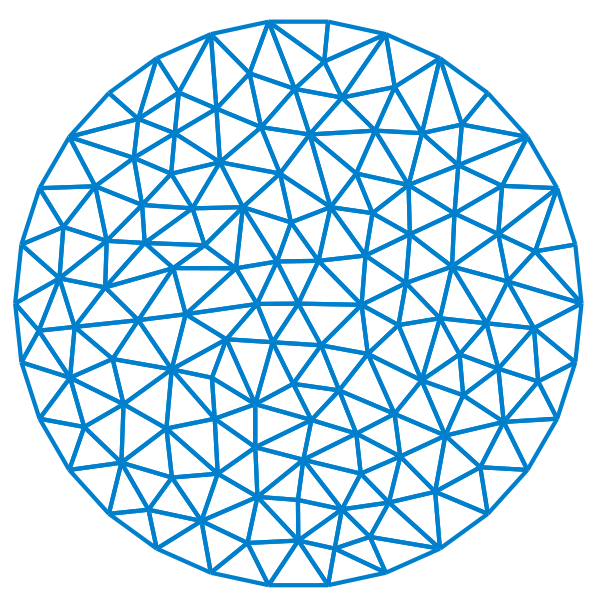
\includegraphics[height=0.20\linewidth]{img/FE_triangulation}
        &
          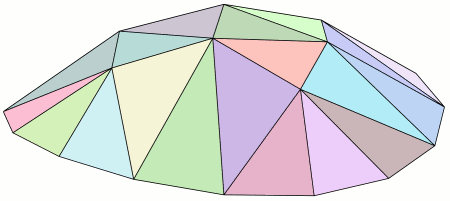
\includegraphics[height=0.15\linewidth]{img/FE_function_3d}
        \\
        {\scriptsize  Triangulation of $\overline\Omega$}
        &
          {\scriptsize Function $u_h \in V_h$ (\P1 approximation)}
      \end{tabular}
    \end{center}

  \item We \alert{approximate the \textbf{variational formulation}} of
    the Poisson problem as follows: find $u_h\in V_h$ such that:
    \begin{BlockNoTitle}
      \vspace{-0.5em}
      \begin{equation*}
        \int_\Omega \grad u_h(\xx) \grad v_h(\xx) d\xx = \int_\Omega f(\xx) v_h(\xx) d\xx \quad \forall v_h\in V_h.
        \label{eq:poisson.variational}
      \end{equation*}
    \end{BlockNoTitle}
  \end{enumerate}
\end{frame}

\begin{frame}
  \begin{theorem}
    Let ${\cal T}_h$ ($h\to 0$) be a sequence of regular meshes of
    $\Omega$. Let $u\in H_0^1(\Omega)$ be the solution of the Poisson
    problem and $u_h\in V_h$ its $\P{k}$ FE approximation. Then
    $$
    \lim_{h\to 0} \norm[H^1(\Omega)]{u-u_h} = 0.
    $$
    Moreover, if $u\in H^{k+1}$ and $k+1>N/2$, then we have the error estimate:
    $$
    \norm[H^1(\Omega)]{u-u_h} \le C \, h^k \, \norm[H^{k+1}(\Omega)]{u}.
    $$
    where $C$ is a constant (independent of $h$ and $u$).
  \end{theorem}
\end{frame}

%%% Local Variables:
%%% coding: utf-8
%%% TeX-master: "numerical-oceanography"
%%% mode: latex
%%% ispell-local-dictionary: "english"
%%% End:


%%,---------------------------------------------------------------------
%%| Ocean Models
%%`---------------------------------------------------------------------
\section[Ocean Models]{Global Circulation Models}
\label{sec:sec-ocean-models}

\begin{sectionframe}
\end{sectionframe}
\begin{frame}{Global circulation models}
%----------------------------------------------------------------------
  \begin{columns}
    \column{0.4\textwidth} {
      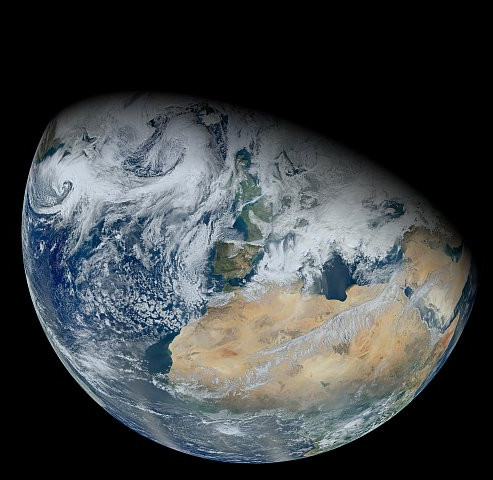
\includegraphics[width=\linewidth]{img/NASA-VIIRS_3Feb2012}
    }
    \column{0.6\textwidth} {
      \begin{itemize}
      \item<1-> \textit{Mathematical} descriptions of general circulation of
        % general circulation of  planetary
        atmosphere and oceans
      \item<2-> Basic components for \textit{climate models}
        \begin{itemize}
        \item Where other equations (e.g. chemical or
          biological) may be coupled
        \end{itemize}
        % \begin{itemize}
        % \item {Weather forecasting, climate understanding, predicting climate evolution...}
        % \end{itemize}
      % \item<3-> Increase of computer power $\Rightarrow$ becoming \textit{more feasible}
       \item<3-> Obtained from simplifications of extremely \textit{complicated
         equations} coming...
         \begin{itemize}
         \item from % different
           conservation laws in physics
           \strip{(momentum, mass, thermodynamics, \\ density, ...)}
         \item on a rotating sphere (the Earth)
         \end{itemize}
      \end{itemize}
      }
  \end{columns}
\end{frame}

\subsection{Quasi-Hydrostatic equations}
%======================================================================

\begin{frame}{The case of (large scale) ocean}
%----------------------------------------------------------------------
  \begin{itemize}\itemsep0.5em
  \item<1> \structure{The ocean:} A slightly compressible fluid
    endowed with Coriolis and buoyancy forces and a set of
    conservation laws from
    Physics
  \item<2-> Simplification of physical laws:\vspace{-1em}
    \begin{columns}
      \column{0.05\linewidth}
      \column{0.41\linewidth}
      \begin{enumerate}\itemsep1.5em
      \item<3-> Boussinesq hypothesis
        \tikz[na] \coordinate(Lboussinesq);
        \hfill
        \tikz[na] \coordinate(Rboussinesq);
      \item<4-> Cartesian coordinates
        \tikz[na] \coordinate(LbetaPlane);
        \hfill
        \tikz[na] \coordinate(RbetaPlane);
      \item<5-> Vertical scaling
        \tikz[na] \coordinate(LverticalScaling);
        \hfill
        \tikz[na] \coordinate(RverticalScaling);
      \end{enumerate}
      \column{0.54\linewidth}
      \begin{overprint}
        \onslide<3>
        \begin{block}{Boussinesq Hypothesis}
          \begin{itemize}
          \item \textit{Density} does not depart from a \textit{mean reference value},
            $\rho_\star>0$.
          \item Then it can be considered constant, $\rho_\star$.
          \item
            Except where it is multiplied by gravity acceleration $g$ (\textit{buoyancy} term)
            % Hence density can be replaced by the constant
            % $\rho_\star$ except in
            % \begin{itemize}
            % \item
              % \textit{buoyancy} term
            % \item conservation of \textit{energy equation}
              % {\color{PHDgrayC} (and state equation)}
          \end{itemize}
        \end{block}
        \onslide<4>
        \begin{block}{Cartesian Coordinates}
          \begin{itemize}
          \item A \textit{local projection} of the Earth surface will be
            assumed
          \item \textit{No loss of generality}: spherical coordinates requires
            only the proper handling of some terms
          \end{itemize}
        \end{block}
        \onslide<5>
        \begin{block}{Vertical Scaling of Domain}
          \vspace{-0.5em}
          \begin{itemize}
          \item The \textit{aspect ratio}
            \begin{equation*}
              \framedmath{\displaystyle\varepsilon = \frac{\text{vertical
                    scales}}{\text{horizontal scales}}}~
                \begin{tabular}[t]{l} is \large\textbf{small} \\[-0.2ex]
                  \tiny\it ~ $10^{-3}$, $10^{-4}$\end{tabular}
            \end{equation*}
%            \pause
          \item Dominant terms can be identified in
            \textit{vertical momentum} equation
          \item Numerical point of view: the problem is
            \textit{rescaled}, obtaining...
            \begin{itemize}
            \item \alert{\textbf{Isotropic domain}}
            \item \alert{\textbf{Anisotropic equations}}
            \end{itemize}
          \end{itemize}
        \end{block}
      \end{overprint}
    \end{columns}
  \end{itemize}

  \begin{tikzpicture}[overlay]
%        \draw<2> [thin, red,opacity=.8, fill=red,fill opacity=0.3](stone) circle (4pt);
%        \path<3>[->,>=latex, PHDredA, shorten >=4pt, opacity=.6]
%        (Lboussinesq) edge [out=0, in=130] (Rboussinesq);
        \draw<3>[->, PHDblue, ultra thick, opacity=.8] (Lboussinesq) -- (Rboussinesq);
        \draw<4>[->, PHDblue, ultra thick, opacity=.8] (LbetaPlane) -- (RbetaPlane);
        \draw<5>[->, PHDblue, ultra thick, opacity=.8] (LverticalScaling) -- (RverticalScaling);
\end{tikzpicture}
\end{frame}


\begin{frame}{The adimensional domain}
%  \vspace*{0.5em}
 After geometrical scaling, we obtain:
   $$
   \domain = \bigl\{ (\xx,z)\in \Rset^{3} \ /\ \xx=(x,y)\in\surface,\
   -D(\xx)< z < 0 \bigr\},
   $$
   where $\surface\subset\Rset^{2}$ is the surface domain and
   $D:\overline\surface \to \Rset_{+}$ a depth function
   \begin{center}
     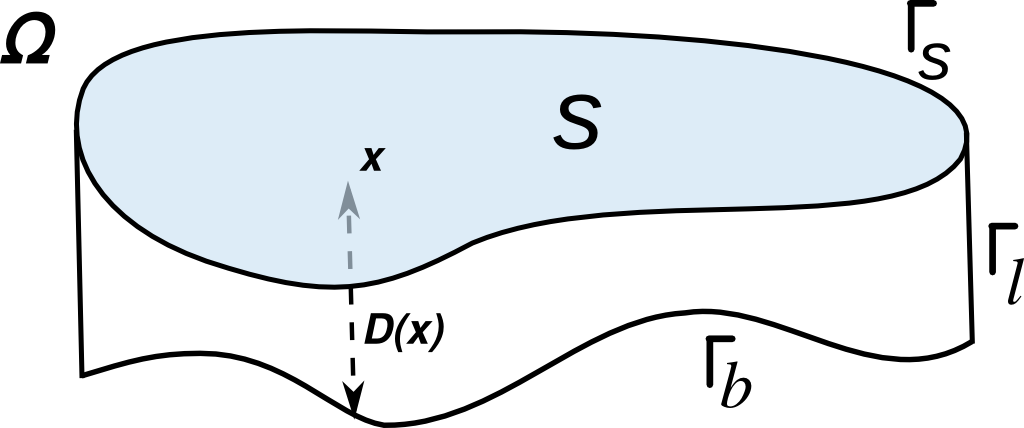
\includegraphics[width=0.4\textwidth, height=5\baselineskip]{img/domain}
   \end{center}
   \begin{itemize}
   \item \alert{Rigid lid hypothesis} (flat surface) is introduced in
     this kind of domains
   \item Notation:
     \begin{itemize}
     \item $\surfaceBoundary$: part of the boundary corresponding to
       the surface
     \item $\bottomBoundary$: part corresponding to the bottom
       boundary
     \item $\talusBoundary$: lateral walls (if any)
     \end{itemize}
   \end{itemize}
 \end{frame}


\begin{frame}{Whole set of Equations}
  %----------------------------------------------------------------------
%  \vspace{-0.2em}
  \note{Comment briefly the main difficulties of Navier--Stokes equations}
  \begin{overprint}
    \onslide<1>
    In the adimensional domain:
    \onslide<2>
    \alert{Aspect ratio}:\tikz[na] \coordinate(LaspectRatio);
    \  multiplying vertical velocity terms!
    \onslide<3>
    \alert{Coriolis} force
    \tikz[na] \coordinate(Lcoriolis);
    \onslide<4>
    \textbf{Coupling} through \alert{\textbf{density}}~
    \tikz[na] \coordinate(Lcoupling);
  \end{overprint}
  \begin{block}{\small Conservation of momentum and continuity}
    \vspace{-0.66\baselineskip}
    \begin{align*}
      \dt \uu + \uu\cdot\gradx\uu + \vv\,\dz\uu  - \Delta_\visc\uu
      + \frac 1 \rho_\star \gradx \pp=
       \tikz[na] \node (Rcoriolis) {\framedmath<3>{\fU}};
      \\
      \tikz[na] \coordinate(RaspectRatio);
        \framedmath<2>{ \varepsilon^2 \Big( \dt \vv + \uu\cdot\gradx\vv +
          \vv\,\dz\vv - \Delta_\visc\vv \Big) }
        \displaystyle
        + \frac 1 \rho_\star \dz \pp +
        \frac{
          \tikz[na] \coordinate(RcouplingA);
          \framedmath<4>{\rho}\,\gravity}{\rho_\star} =
        0\hskip+0.5em
      \\[-0.2em]
      \div\uu + \dz\vv = 0\hskip+0.5em
    \end{align*}
    \vspace{-1.4\baselineskip}
  \end{block}
  \begin{block}{\small Convection-diffusion of \textit{temperature} and
      \textit{salinity} + state equation (density)}
    \vspace{-0.66\baselineskip}
    \begin{align*}
      \dt \Te  + (\uu \cdot \gradx) \Te + (\vv\cdot\dz) \Te  - \nu_\Te\Delta \Te &= \fT
      \\[0.3em]
      \dt \Sa  + (\uu \cdot \gradx) \Sa + (\vv\cdot\dz) \Sa -
      \nu_\Sa\Delta \Sa &= \fS
      \\[0.3em]
      \tikz[na] \coordinate(RcouplingB);
      \framedmath<4>{\rho} = \rho_\star\big(1-\beta_\Te(\Te-\Te_\star) + \beta_\Sa(\Sa&-\Sa_\star)\big)
    \end{align*}
    \vspace{-1.4\baselineskip}
  % \item Equation of state (dependence of density in terms of
  %   temperature and salinity)
  %   where $\Te_\star$ and $\Sa_\star$ are given reference values.
  \end{block}
  \tikzstyle{RaspectRatio} = [draw, circle, minimum size=.5cm, node
  distance=1.75cm]
  \tikzstyle{redcircle} = [draw, circle, color=PHDredA, node distance=3cm,
  minimum height=2em]

  \begin{tikzpicture}[overlay]
    \path<2>[myarrow]
    (LaspectRatio) edge [out=320, in=130] (RaspectRatio);
    \path<3>[myarrow]
    (Lcoriolis) edge [out=0, in=130] (Rcoriolis);
    \path<4>[myarrow]
    (Lcoupling) edge [out=0, in=135] (RcouplingA);
    \path<4>[myarrow]
    (Lcoupling) edge [out=0, in=135] (RcouplingB);
        % \draw<3>[->, PHDblue, ultra thick, opacity=.8] (Lboussinesq) -- (Rboussinesq);
        % \draw<4>[->, PHDblue, ultra thick, opacity=.8] (LbetaPlane) -- (RbetaPlane);
        % \draw<5>[->, PHDblue, ultra thick, opacity=.8] (LverticalScaling) -- (RverticalScaling);
  \end{tikzpicture}
\end{frame}


\begin{frame}{The case of constant density}
  %----------------------------------------------------------------------
  In the first part of this work, we fix the following usual
  assumption:

  \begin{center}
    \alert{density is a known constant}, e.g. $\rho=\rho_\star>0$
  \end{center}
  \vspace*{0.66em}
  \begin{itemize}\itemsep0.6em
  \item<1-> Then fluid motion equations can be treated independently
  \item<2-> If \tikz[na] \node (LrhoG) {$\rho g$};
    is written as potential... then
    \uncover<3->{it can be absorbed by pressure
      \tikz[na] \coordinate(LpressureAbsorb);}

  \begin{overprint}
    \onslide<1>
    \begin{block}{\small Conservation of momentum and continuity}
      \vspace{-1.3\baselineskip}
      \begin{align*}
        \dt \uu + \uu\cdot\gradx\uu + \vv\,\dz\uu - \Delta_\visc\uu +
        \frac 1 \rho_\star \gradx \pp &= \fU
        \\
        \tikz[na] \coordinate(RaspectRatio); \varepsilon^2 \Big( \dt \vv
        + \uu\cdot\gradx\vv + \vv\,\dz\vv - \Delta_\visc\vv \Big)
        + \dz \pp
        + \rho\gravity
        &= 0
        \\
        \div\uu + \dz\vv &= 0
      \end{align*}
      \vspace{-1.4\baselineskip}
    \end{block}
    \onslide<2>
    \begin{block}{\small Conservation of momentum and continuity}
      \vspace{-1.3\baselineskip}
      \begin{align*}
        \dt \uu + \uu\cdot\gradx\uu + \vv\,\dz\uu - \Delta_\visc\uu +
        \gradx \pp= \fU
        \\
        \varepsilon^2 \Big( \dt \vv
        + \uu\cdot\gradx\vv + \vv\,\dz\vv - \Delta_\visc\vv \Big)
        + \dz \pp +
%        \tikz[na] \coordinate;
        \tikz[na] \node[draw, circle, color=PHDredA, fill
        opacity=1] (RrhoG) {$\rho\gravity$};
        = 0
        \\
        \div\uu + \dz\vv = 0
      \end{align*}
      \vspace{-1.4\baselineskip}
    \end{block}
    \onslide<3->
    \begin{block}{\small Conservation of momentum and continuity}
      \vspace{-1.3\baselineskip}
      \begin{align*}
        \dt \uu + \uu\cdot\gradx\uu + \vv\,\dz\uu - \Delta_\visc\uu +
        \gradx \pp= \fU
        \\
        \varepsilon^2 \Big( \dt \vv + \uu\cdot\gradx\vv + \vv\,\dz\vv -
        \Delta_\visc\vv \Big)
        +
        \tikz[na] \node[draw, circle, color=PHDredA, fill opacity=1]
        (RpressureAbsorb) {$\dz \pp$}; = 0
        \\
        \div\uu + \dz\vv = 0
      \end{align*}
      \vspace{-1.4\baselineskip}
    \end{block}
  \end{overprint}
  \vspace{0.66em}
\item<4-> This system will be called anisotropic equations...
  \end{itemize}

  \begin{tikzpicture}[overlay]
    \path<2>[->,>=latex, PHDredA, shorten >=4pt, opacity=.6, thick]
    (LrhoG) edge [out=-45, in=135] (RrhoG);
    \path<3>[->,>=latex, PHDredA, shorten >=4pt, opacity=.6, thick]
    (LpressureAbsorb) edge [out=-45, in=45] (RpressureAbsorb);
  \end{tikzpicture}
 \end{frame}

\begin{frame}{Anisotropic Navier--Stokes equations}
  %----------------------------------------------------------------------
  % \vspace*{0.5em}
  \begin{BlockNoTitle}
    \begin{tabular}{@{}l|>{$}r<{$}>{$}l<{$}@{}}
      \multirow{3}{*}{
        \begin{turn}{30}
          \small\aniNS
        \end{turn}
        }
        &
        \dt \uu + \alert<2>{\uu\cdot\gradx\uu + \vv\,\dz\uu} - \Delta_\visc\uu +
        \gradx \pp &= \fU
        \\[0.2em]&
        \varepsilon^2 \Big( \dt \vv + \alert<2>{\uu\cdot\gradx\vv + \vv\,\dz\vv} -
        \Delta_\visc\vv \Big)
        + \dz \pp &= 0
        \\[0.2em]&
        \div\uu + \dz\vv &= 0
      \vspace{-1.4\baselineskip}
    \end{tabular}
  \end{BlockNoTitle}
  \uncover<2-> {If $\varepsilon=1$, we get standard $O(1)$ \alert<2>{Navier--Stokes} equations
  \par  \hfill
  ...but $\varepsilon=1$ is  not realistic in geophysical domains (\exclamation)}
  \vfill
  \uncover<3->{
  Better approaches:}
  \begin{enumerate}\itemsep0.5em
  \item<3-> $\varepsilon=0$: Hydrostatic Navier--Stokes or Primitive Equations
  \item<4-> $0<\varepsilon\lesssim 10^{-3}$:
    ``\textit{\bfseries\alert{Quasi-hydrostatic}}'' Navier--Stokes Equations
    \vspace*{0.5em}
    \begin{itemize}
    \item<4-> More realistic case in geophysical domains, e.g.
      $$
      \varepsilon = \frac{\text{5,121 m}}{\text{3,700 km}}
      \quad
      \text{(Mediterranean Sea)}
      $$
    \end{itemize}
  \end{enumerate}
\end{frame}

\begin{frame}{Hydrostatic Navier--Stokes (or Primitive) equations}
%------------------------------------------------------------
  The simplification \framedmath{\varepsilon=0} is usually taken,
  obtaining:
\begin{block}{}
  \begin{tabular}{@{}l|>{$}r<{$}>{$}l<{$}@{}}
    \multirow{3}{*}{
      \begin{turn}{30}
        \small \hydNS
      \end{turn}
    }
    &
    \dt\uu + (\uu\cdot\gradx)\uu +\vv\dz \uu
    - \Delta_\visc\uu + \gradx\pp &= \ff \ \In\domain,
    \label{eq:HNS.a}
    \\
    &
    \dz\pp & = 0 \ \In\domain,
    \label{eq:HNS.b}
    \\
    &
    \divx\uu +  \dz\vv &= 0 \ \In\domain.
    \label{eq:HNS.c}
  \end{tabular}
\end{block}
\begin{itemize}
\item Originally derived from scale analysis~\cita{Pedlosky:1987,CushmanRoisin-Beckers:09}
\item Mathematically justified as limit of anisotropic Navier--Stokes \aniNS,
  when $\varepsilon\to 0$ in vertical momentum
  equation~\cita{Besson-Laydi:92,Azerad-Guillen:01}
% \item Complemented with adequate boundary
%   conditions.
% ~(\ref{eq:bc.1})--(\ref{eq:bc.3}). See that, now,
%   it is natural not imposing boundary conditions for $\vv$ on
%   $\talusBoundary$.
\end{itemize}
\end{frame}

% \begin{frame}{Vertical integration of Hydrostatic Navier--Stokes}
%   \begin{itemize}
%   \item Model widely studied (both theoretically and in numerical
%     simulations)
%   \item Almost all works use the following \emph{\structure{vertical integrated formulation
%           of the primitive equations}}: find $\uu:\domain\times (0,T)
%       \to \Rset^2$, horizontal velocity, and $\ps:\domain\times (0,T)
%       \to\Rset$, (artificial) surface pressure, such that
%       \begin{BlockNoTitle}
%         \begin{tabular}{@{}l|>{$}r<{$}>{$}l<{$}@{}}
%           \multirow{3}{*}{
%             \begin{turn}{30}
%               \small\reducedProblem
%             \end{turn}
%           }
%           &
%           \dt\uu + (\uu\cdot\gradx)\uu +\vv\dz \uu - \Delta_\visc\uu +
%           \gradx\ps = \ff & \In\domain,
%           \label{eq:EP.a}
%           \\
%           &
%           \divx\langle\uu\rangle = 0 & \In\domain,
%           \label{eq:EP.b}
%           \\
%           &
%           \uu = 0 \quad \On\bottomBoundary\cup\talusBoundary, \qquad
%           \visc_z\dz\uu = \gs &\On \surfaceBoundary,
%           \label{eq:EP.c}
%         \end{tabular}
%       \end{BlockNoTitle}
%       where $\vv$ and $\langle\uu\rangle$ are defined by:
%   $$
%   \vv(\xx,\zz,t) = \int_z^0 \divx\uu(\xx,s,t)\;ds, \qquad
%   \langle\uu\rangle(\xx,t) = \int_{-D(\xx)}^0 \uu(\xx,\zz,t) dz.
%   $$
%       \begin{itemize}
%     \item Integrate in $z$ the divergence equations in ~\hydNS
%     \item Use account the rigid lid hypothesis~(\ref{eq:bc.2})
%     \end{itemize}
%     we obtain the
%       next equivalent
% \end{itemize}
% \end{itemize}
% \end{frame}

\begin{frame}{Vertical integration of Hydrostatic Navier--Stokes}
  \begin{itemize}\itemsep0.77ex
  \item Widely studied \soften{(both theoretically and in numerical
    simulations)}
  \item Almost all works \soften{use the following equivalent}
    \textbf{\alert{vertical integrated formulation of the primitive
        equations}}:
    \begin{itemize}
    \item find $\uu:\domain\times (0,T) \to \Rset^2$ (horizontal
      velocity) and
    \item $\ps:\surface\times (0,T) \to\Rset$ (artificial surface
      pressure) such that
    \end{itemize}
    \begin{BlockNoTitle}
      \begin{tabular}{@{}l|>{$}r<{$}>{$}l<{$}@{}}
        \multirow{3}{*}{
          \begin{turn}{30}
            \small\reducedProblem
          \end{turn}
        }
        &
        \dt\uu + (\uu\cdot\gradx)\uu +\vv\dz \uu - \Delta_\visc\uu +
        \gradx\ps = \ff & \In\domain,
        \label{eq:EP.a}
        \\
        &
        \divx\langle\uu\rangle = 0 & \In\domain,
        \label{eq:EP.b}
        \\
        &
        \uu = 0 \quad \On\bottomBoundary\cup\talusBoundary, \qquad
        \visc_z\dz\uu = \gs &\On \surfaceBoundary,
        \label{eq:EP.c}
      \end{tabular}
    \end{BlockNoTitle}
    where $\vv$ and $\langle\uu\rangle$ are defined by:
    \vspace{-0.5em}
    $$
    \vv(\xx,\zz,t) = \int_z^0 \divx\uu(\xx,s,t)\;ds, \qquad
    \langle\uu\rangle(\xx,t) = \int_{-D(\xx)}^0 \uu(\xx,\zz,t) dz.
    $$
  \item It is obtained...
    \begin{itemize}
    \item Integrating in $z$ the divergence equations in ~\hydNS
    \item Using the \textbf{rigid lid hypothesis}
    \end{itemize}
  \end{itemize}
\end{frame}

\begin{frame}
\frametitle{Comparison of the models}
\vspace{0.5em}
\small
\begin{tabularx}{\textwidth}{@{}X@{\qquad}X@{}}
  {\bf Integrated model \reducedProblem} &
  {\bf Not integrated \aniNS}
  \\ \toprule
  System of \textit{3 PDE} + 3 unknowns: \ \good&
  System of  \textit{4 PDE} +   4 unknowns: \ \bad
  \\ %\midrule
    % 3 unknowns\ \good\ :
    \hspace{17ex}
    \begin{tabular}[b]{l}
      $\uu$ (in $\domain$) \\ $\ps$ (in $\surface$) \ \good
    \end{tabular}
    &
  % 4 unknowns \bad \ :
      \hspace{17ex}
      \begin{tabular}[l]{l}
      $\uu$ (in $\domain$), \\  $\vv$ (in $\domain$),
      \\ $\pp$ (in $\domain$) \ \bad
    \end{tabular}
    % $\vv=\vv(\uu)$
    \\ \midrule
    $\vv=\vv(\uu)$ is \emph{decoupled} \ \good
    &
    $\vv$ is \textit{not decoupled}\ \bad
  \\ \midrule
   Differential
  $+$ z-\emph{integral} pb. \ \bad
  &
  Only differential problems \ \good
  \\ \midrule
  Structured meshes\ \bad
  &
  Unstructured or struct. meshes \ \good
  \\
  % \begin{center}\vspace{-2em}
  \hspace{-3.2ex}
    \hfill\pgfimage[width=3.5cm]{img/struct-mesh}\hfill\qquad~
  % \end{center}
%  \\ \bottomrule
    &
  % \begin{center}\vspace{-2em}
  \hspace{-3.2ex}
    \hfill\pgfimage[width=3.5cm]{img/unstruct-mesh}\hfill\qquad~
  % \end{center}
    \\ \hline
    Needs simplification $\varepsilon=0$\ \bad
    &
    More general models, $\varepsilon\ge 0$\ \good
  \\ \midrule
  {\scriptsize Less flexibility for include extensions} \bad
  &
  {\scriptsize Flexibility (extensions like mesh adaptivity)}\good
\end{tabularx}
\end{frame}

% \begin{frame}
% \frametitle{Comparison of the models}
% \vspace{0.5em}
% \small
% \begin{tabularx}{\textwidth}{@{}X@{\qquad}X@{}}
%   {\bf Not integrated \aniNS}  & {\bf Integrated model \reducedProblem}
%   \\ \toprule
%   System of  4 PDE +   4 unknowns: \ \bad &
%   System of 3 PDE + 3 unknowns: \ \good
%   \\ %\midrule
%   % 4 unknowns \bad \ :
%       \hspace{17ex}
%       \begin{tabular}[l]{l}
%       $\uu$ (in $\domain$), \\  $\vv$ (in $\domain$),
%       \\ $\pp$ (in $\domain$) \ \bad
%     \end{tabular}
%     % $\vv=\vv(\uu)$
%     &
%     % 3 unknowns\ \good\ :
%     \hspace{17ex}
%     \begin{tabular}[b]{l}
%       $\uu$ (in $\domain$) \\ $\ps$ (in $\surface$) \ \good
%     \end{tabular}
%     \\ \midrule
%     $\vv$ is not decoupled\ \bad
%     &
%     $\vv=\vv(\uu)$ is decoupled \ \good
%   \\ \midrule
%   Only differential problems \ \good  &  Differential
%   $+$ z-integral pb. \ \bad
%   \\ \midrule
%   Unstructured or struct. meshes \ \good &
%   Structured meshes\ \bad
%   \\
%   % \begin{center}\vspace{-2em}
%   \hspace{-3.2ex}
%     \pgfimage[width=3.5cm]{img/unstruct-mesh}
%   % \end{center}
%   &
%   % \begin{center}\vspace{-2em}
%   \hspace{-3.2ex}
%     \pgfimage[width=3.5cm]{img/struct-mesh}
%   % \end{center}
% %  \\ \bottomrule
%     \\ \hline
%     More general models, $\varepsilon\ge 0$\ \good &
%     Needs simplification $\varepsilon=0$\ \bad
%   \\ \midrule
%   {\scriptsize Flexibility (extensions like mesh adaptivity)}\good &
%   {\scriptsize Less flexibility for include extensions} \bad
% \end{tabularx}
% \end{frame}

\begin{frame}{Our objectives}
\begin{enumerate}\itemsep0.66em
\item \textit{Analysis} of the pecularities (the stability) of
  Navier--Stokes in geophysical domains (where $\varepsilon$ is ``small'')
\item Use this analysis to \textit{propose some new FE
    combinations} which:% fulfill the following \textit{purposes}:
  \begin{enumerate}\itemsep0.33em
  \item Allow numerically solving \textit{more realistic models than pure hydrostatic
      ones}. Moreover, to achieve solving both Hydrostatic and not
    Hydrostatic Navier--Stokes equations in the same way.
  \item \textit{Avoid the introduction of integro-differential equations},
    exploiting the advantages of non-integral models (enounced above)
  \end{enumerate}
\item Develop \textit{new discrete schemes} which are
  stable, when $\varepsilon\to 0$, for usual LBB FE combinations for
  Navier--Stokes (including $\varepsilon=0$)
\item Extend these new schemes to \textit{more complex time-dependent
    problems} (including variable density) and define \textit{new
  time-splitting schemes}
\end{enumerate}
\end{frame}


%%% Local Variables:
%%% coding: utf-8
%%% TeX-master: "numerical-oceanography"
%%% mode: latex
%%% ispell-local-dictionary: "english"
%%% End:


%%,---------------------------------------------------------------------
%%| Stokes Hydrostatic Stable FE combinations}
%%`---------------------------------------------------------------------
\section{New Stokes FE which are Hydrostatic--Stable}
\label{sec:hydr-stable-fe}

\begin{sectionframe}
  \vfill
  \begin{abstract}
    \begin{enumerate}
    \item Analysis of \textbf{Hydrostatic Stokes} equations show that
      they are \alert{not stable for ``classical'' Stokes LBB-stable FE
      combinations}. The reason is:
      \begin{itemize}
      \item An additional inf-sup condition is required
      \item It imposes richer FE spaces for horizontal velocity than
        vertical one
        % \begin{enumerate}
        % \item Usual Stokes LBB inf-sup condition
        % \item An additional ``hydrostatic'' inf-sup condition
        % \end{enumerate}
      \end{itemize}
    \item Stability analysis of \alert{classical Stokes} equations when
      unequal FE spaces are used for each component of the  velocity
    \item We provide some \textbf{new elements} which are
      \alert{stable for Hydrostatic Stokes} Equations
    \end{enumerate}
  \end{abstract}
\end{sectionframe}

% \subsection{Stability of Hydrostatic Stokes}
% %----------------------------------------------------------------------

% \begin{sectionframe}
%   \vfill
%   \begin{abstract}
%     \begin{enumerate}
%     \item<alert@*> Analysis of \textbf{Hydrostatic Stokes} equations.
%       They are \alert{not stable for ``classical'' Stokes LBB-stable FE
%       combinations}. The reason is:
%       \begin{itemize}
%       \item An additional inf-sup condition is required
%       \item It imposes richer FE spaces for horizontal velocity than
%         vertical one
%         % \begin{enumerate}
%         % \item Usual Stokes LBB inf-sup condition
%         % \item An additional ``hydrostatic'' inf-sup condition
%         % \end{enumerate}
%       \end{itemize}
%       \pgfsetfillopacity{0.33}
%     \item {\textbf{Stability analysis of classical Stokes} equations when
%       unequal FE spaces are used for each component of the  velocity}
%     \item We provide some \textbf{new elements which are
%       stable} for the Hydrostatic Stokes Equations
%     \end{enumerate}
%   \end{abstract}
% \end{sectionframe}

\begin{frame}{Numerical Experiment}
  \textbf{Stable FE approximations for Stokes} equations in a domain
  $$\alert{\Omega_{\epsilon}} = (0,1)\times(0,\alert{\varepsilon}) \subset \Rset^2$$
  \vspace{-1.2em}
  \begin{itemize}
    \setlength{\itemsep}{0.5em}
  \item Standard \structure{lid-driven cavity test}:
    \begin{itemize}
      \itemsep0.3em
    \item $v=0$ on $\Gamma_S\cup \Gamma_B$
    \item $u=0$ on $\Gamma_l \cup \Gamma_B$, traction B.C. on surface.
    \end{itemize}
  \item What happens if \structure{$\varepsilon \to 0$}? \hfill Test:
    $\varepsilon=1,10^{-1},10^{-2},\dots,10^{-5}$).
  \end{itemize}
  \medskip
  \textbf{Equivalently}: solving in the \textbf{unit square}
  $$\alert{\Omega} = (0,1)\times(0,1) \subset \Rset^2$$
  \vspace{-1.5em}
  \begin{BlockNoTitle}
    \begin{tabular}{@{}l|>{$}r<{$}>{$}l<{$}@{}}
      \multirow{3}{*}{
        \begin{turn}{30}
          \small\aniStokes
        \end{turn}
        }
        &
        - \Delta u + \gradx \pp &= 0 \quad \text{ in } \Omega
        \\[0.2em]&
        -\varepsilon^2
        \Delta v + \dz \pp &= 0 \quad \text{ in } \Omega
        \\[0.2em]&
        \divx u + \dz\vv &= 0 \quad \text{ in } \Omega
      \vspace{-1.4\baselineskip}
    \end{tabular}
  \end{BlockNoTitle}
\end{frame}

\begin{frame}{Usual FE are not valid for \aniNS when $\varepsilon\to 0$}
  \vspace*{0.25em}
  \begin{itemize}\itemsep0.33em
  \item Example: \P2-\P1 cavity test when $\varepsilon\to 0$
    \hfill{\small $\varepsilon=1,...,10^{-5}$)}
  \item \myframed{\textbf{Instabilities} when $\varepsilon\lesssim
      10^{-3}$ \hspace{5.2em}..due to vertical velocity}
    \note{Instabilities are due to anisotropy in domain (or in equations)}
  \end{itemize}
  \vspace*{0.25em}
  \begin{columns}
    ~\hspace{2em}
    \column{0.6\linewidth}
    \PlayVideoWithLabel[0.9\linewidth][0.85\linewidth][Streamlines]{%
      video/eps-to-zero-P2-P1-streamlines-20s.avi}
    \column{0.4\linewidth}
    \centering\PlayVideoWithLabel[0.62\linewidth][0.62\linewidth][Horizontal
    \ $\uu$]{%
      video/eps-to-zero-P2-P1-u-20s.avi}
    \\[0.3em]
%    \par\vskip-0.62em
    \centering\PlayVideoWithLabel[0.62\linewidth][0.62\linewidth][Vertical
    \ $\vv$]{%
      video/eps-to-zero-P2-P1-v-20s.avi}
    \end{columns}
  % \begin{center}
  %   \PlayVideoWithLabel[0.5\linewidth][0.5\linewidth][Streamlines]
  %   {video/eps-to-zero-P2-P1-streamlines.avi}
  % \end{center}
  \begin{flushright}
  \end{flushright}
\end{frame}


\begin{frame}{Why does the above occurs?}
\framesubtitle{A first approach}

\begin{itemize}\itemsep0.66em
\item We fix \textbf{the most unfavorable case}: $\varepsilon=0$

\item Let us define the spaces (which reflect \textit{boundary conditions}):
  \begin{equation*}
    \UU=\Uspace,\quad \VV=\Vspace,\quad \PP=\Pspace.
    \label{eq:spaces}
  \end{equation*}
\item And consider the (linear steady) hydrostatic
  Stokes problem:%
  \note{See that it's the kind of problem that arises when
    performing time discretizations of \hydNS}%
  % (``adequate spaces'') such that: = \Uspace\times
  % \Vspace\times\Pspace$ s.t.
  \begin{align*}
    &\text{Find } (\uu,v,p) \in U\times V \times P,
    \\
%  \qquad\qquad
  &\text{\hydStokes}
  \left\{
    \begin{aligned}
      - \visc_\xx\Delta\uu + \gradx\pp &= \ff_\xx &
      \begin{overprint}
        \onslide<2> \llaveizq{
          \alert{$\uu$: only primal variable}\\
          \alert{$\pp, \vv$: Lagrange multipliers}}
        \onslide<3>$\leftarrow \times\ \alert{\bar \uu \in \Uspace}$
      \end{overprint}
      \\ \dz\pp & =0 &
      \begin{overprint}
        \onslide<2>$\leftarrow \alert{\text{2nd. restriction}}$
        \onslide<3>$\leftarrow \times\ \alert{\bar v \in \Vspace}$
      \end{overprint}
      \\[0.1em]
      \divx\uu + \dz\vv &= 0 &
      \begin{overprint}
        \onslide<2>$\leftarrow \alert{\text{1st. restriction}}$
        \onslide<3>$\leftarrow \times \ \alert{\bar p \in \Pspace}$
      \end{overprint}
      \\
      +\ &\text{b. c.}
    \end{aligned}
  \right.
\end{align*}
\end{itemize}
\end{frame}



\begin{frame}{Analysis of the continuous problem}
% Find $(\uu,v,p) \in U\times V \times P =
% \Uspace\times\Vspace\times\Pspace$,
Weak formulation:
\begin{equation*}
  \left\{
    \begin{aligned}
      \visc_\xx\big(\grad u,\grad\bu\big)
      -\big(\divx\bu, p\big) &= \big(\ff_\xx,\bu\big) && \forall
      \bu\in \UU=\Uspace,
      \\
      \big(\divx \uu + \dz v,\bp\big) & \alert<2>{= 0} &&
      \forall\bp\in \PP=\Pspace
      \\
      \big(\dz \bv, p\big) & =0 &&
      \forall\bv\in \VV=\Vspace
    \end{aligned}
  \right.
\end{equation*}
\pause
Two Inf-Sup conditions are suggested:
\begin{alignat*}{4}
  \label{eq:ISp}
  \tag*{\ensuremath{(IS)^\PP}\xspace}
  &\quad&
  \sup_{0\neq(\uu,\vv)\in \UU \times \VV}
  \frac{(\div(\uu,\vv),\pp)}{\|\grad \uu,\dz \vv\|}
  &\ge \ConstISp \|\pp\|
  &\quad&
  \forall \pp \in \PP,
  \\
  \label{eq:ISv}
  \tag*{\ensuremath{(IS)^\VV}\xspace}
  &\quad &
  \sup_{0\neq \pp \in \PP}
  \frac{(\dz \vv,\pp)}{\|\pp\|}
  &\ge \ConstISv \|\dz\vv\|
  &\quad&
  \forall \vv\in \VV
\end{alignat*}

\begin{remark}
  \begin{itemize}
  \item \ISp: similar to Stokes LBB
    inf-sup condition (weaker?)~\cite{Brezzi-Fortin:91}
  \item \ISv: a new condition, first introduced by
    \textbf{P.~Azerad}~\cite{Azerad:1994,Azerad:PhD:96}
  \end{itemize}
\end{remark}
\bigskip~
% \begin{equation*}
%   \begin{aligned}
%     \ISp\ & \alert<2>{
%       \sup_{0\neq( \uu, v)\in U\times V}
%       \frac{\big(\divx \uu +\dz v, p\big)}{||\grad \uu||_0 + ||\dz v||_0}
%       \ge
%       \beta_1 ||p||_0 \quad \forall p \in P
%     }
%     \\
%     \uncover<3->{
%       \ISv\ & \alert<3>{
%         \sup_{0\neq p\in P}
%         \frac{(\dz v, p)}{||p||_0}
%         \ge
%         \beta_2
%         ||\dz v||_0 \quad \forall v \in V
%       }
%     }
%   \end{aligned}
% \end{equation*}
\end{frame}

\begin{frame}{Existence, uniqueness and energy estimates}

  \begin{lemma}
    \ISp and \ISv are satisfied
  \end{lemma}
  \textbf{Proof}:
  \begin{itemize}
  \item \ISp $\Leftarrow$ Stokes inf-sup.
  \item \ISv for $v\in \Vspace$, take $p=\dz v\in \Pspace$
  \end{itemize}


  % Thanks \ISp and \ISv, we can provide an existence result,
  % \textit{not based on the reduced formulation} of \hydStokes:

\vfill

\begin{theorem}
  \begin{itemize}
  \item There exists an unique weak solution $(\uu,v,p)\in
    \UU\times\VV\times\PP$ of \hydStokes.
  \item
    Moreover, the following continuous dependence estimates hold:
    \begin{equation*}
      \label{eq:stability.estimates}
      \begin{aligned}
        ||\grad\uu||_0 \le ||\ff||_{-1}, && ||\dz\vv||_0 \le
        \frac{1}{\beta_2}||\ff||_{-1}, && ||p||_0 \le \frac{2}
        {\beta_1}||\ff||_{-1}
      \end{aligned}
    \end{equation*}
  \end{itemize}
  \label{theorem:1}
\end{theorem}
\end{frame}

\SetEmptyBackground
\begin{frame}
  \begin{proof}[Proof (P. Azerad~\cite{Azerad:PhD:96})]
    \begin{itemize}
    \item \structure{\textit{Step 1}}.
      Consider
      $\XX=\UU\times\VV\times\PP$ and, for each
      $\cc=(\uu,\vv,\pp)\in \XX$ and $\bc = (\bu, \bv, \bp)\in
      \XX$, \textit{define the forms}:
      \begin{align}
        \AA(\cc,\bc) & = \product{\grad \uu, \grad\bu} -
        \product{p,\div(\bu, \bv)} - \product{\div(\uu,v),\bp},
        \label{eq:HSoperator}
        \\
        \LL(\cc) & = \langle f,\bu \rangle,
        \label{eq:HSlinearform}
      \end{align}
      \begin{flushleft}
        \color{PHDgray}{
        \small \quad  $\hookrightarrow$ \textit{Notation}:
        $(\cdot,\cdot) \equiv  L^2(\domain)$ product, \
        $\langle\cdot,\cdot\rangle \equiv \UU^{-1}\times\UU$
        }
      duality.
      \end{flushleft}

      Then the weak formulation
      \hydStokes\ can be written as:
      \begin{equation}
        \label{eq:HS.weak.formulation}
        \text{Find}\ \cc\in \XX \quad\text{such that}\quad
        \AA(\cc,\bc) = \LL(\bc),
        \quad \forall \bc \in \XX.
      \end{equation}

    \item \structure{\textit{Step 2}}.
      Then, \ISp + \ISv $\Rightarrow$ ``\textit{generalized coercivity}'' for
      $\AA$ $\Rightarrow$ existence, uniqueness and bounds.
    \end{itemize}
  \end{proof}
\end{frame}
\SetDefaultBackground


\SetEmptyBackground
\begin{frame}
  \begin{proof}[A new proof  (via the \emph{saddle point}
     framework)]
%  Saddle point theory
  \begin{itemize}
  \item Let $\WW=\UU\times\VV$ endowed with
    $\|\ww\|_\WW=\|\nabla\uu,\dz\vv\|$
  \item Hydrostatic Stokes Problem $\equiv$ find $\ww \in \WW$
    and $\pp\in\PP$ such that
    \begin{align}
      \label{eq:saddle.point.proof.1}
      a(\ww,\bw) + b(\bw, p) &= \langle (\ff,0)^t,\bw \rangle_{\WW',\WW}  \quad\forall \bw \in \WW,
      \\
      \label{eq:saddle.point.proof.2}
      b(\ww,\bp) &=0  \quad\forall \bp\in \PP,
    \end{align}
    where, for each $\ww=(\uu,v)$ and $\bw = (\bu,\bv) \in \WW$:
    \begin{equation*}
      \begin{aligned}
        &a:\WW \times \WW \to \Rset, && a(\ww,\bw ) = \product{\grad
          \uu, \grad\bu} \leftarrow\text{\alert{\bf\itshape Not
            coercive} on } \UU\times\VV\exclamation
        \\
        &b:\WW \times \PP \to \Rset, && b(\ww,p) = -\product{\divx\uu
          + \dz\vv, p}
      \end{aligned}
    \end{equation*}
    \item But for well-posedness
      of~(\ref{eq:saddle.point.proof.1})--(\ref{eq:saddle.point.proof.2})
      it is sufficient$^*$ (see~\cite{Brezzi-Fortin:91}):
      \vspace{0.4em}
      \begin{enumerate}\itemsep0.4em
      \item $\displaystyle
          \sup_{\ww\in \WW}
          \frac{b(\ww,p)}{||\ww||_\WW} \ge \beta_0 ||p||_{P/\ker B^t},
          \quad\forall\pp\in\PP$
          \hfill $\leftarrow$ \ISp \qquad~
        \item $a(\cdot,\cdot)$ is \alert{\textbf{\itshape coercive on} $\ker B$}
          \hfill
        $\leftarrow$ \ISv \qquad~
      \end{enumerate}
    \end{itemize}
    \scriptsize{$^*$\color{PHDgrayB}{where $B: \WW \to \PP',\ \product{B\ww,p} =
          b(\ww,p) =\product{\ww,B^t p}$}}%
\end{proof}
\end{frame}
\SetDefaultBackground

\begin{frame}{The discrete problem}
  \begin{itemize}
  \item Let $\Uh$, $\Vh$, $\Ph$
    be conforming $\Uspace$, $\Vspace$, $\Pspace$ \
    finite element spaces
    on a (possibly unstructured) mesh ${\cal T}_h$
  \item Discrete problem: find $(\uu,v,p) \in \Uh\times \Vh \times \Ph$
    such that
\begin{equation*}
  \hydStokesDiscr
  \left\{
    \begin{aligned}
      \visc_\xx\product{\grad \uu,\grad\bu}
      -\product{\divx\bu, p} &= \product{f_\xx,\bu} && \forall
      \bu\in U_h,
      \\
      \product{\dz \bv, p} & =0 &&
      \forall\bv\in V_h,
      \\
      \product{\divx \uu + \dz v,\bp} & = 0 &&
      \forall\bp\in P_h.
    \end{aligned}
  \right.
\end{equation*}

  \item Let us define the discrete inf-sup conditions:
\begin{alignat*}{4}
  \tag*{\ensuremath{(IS)^\PP_h}\xspace}
  \label{eq:ISph}
  &\quad&
  \sup_{0\neq(\uh,\vh)\in \Uh \times \Vh}
  \frac{(\div(\uh,\vh),\ph)}{\|\grad \uh,\dz \vh\|}
  &\ge \ConstISph \|\ph\|
  &\quad&
  \forall \ph \in \Ph,
  \\
  \tag*{\ensuremath{(IS)^\VV_h}\xspace}
  \label{eq:ISvh}
  &\quad &
  \sup_{0\neq \ph \in \Ph}
  \frac{(\ph,\dz \vh)}{\|\ph\|}
  &\ge \ConstISvh \|\dz\vh\|
  &\quad&
  \forall \vh\in \Vh,
\end{alignat*}
%    \begin{equation*}
%   \begin{aligned}
%     \ISph\ &
%       \sup_{0\neq( \uu, v)\in U_h\times V_h}
%       \frac{\product{\divx \uu +\dz v, p}}{||\grad \uu||_0 + ||\dz v||_0}
%       \ge
%       \gamma_1 ||p||_0 \quad \forall p \in P_h
%     \\
%       \ISvh\ &
%         \sup_{0\neq p\in P_h}
%         \frac{\product{\dz v, p}}{||p||_0}
%         \ge
%         \gamma_2
%         ||\dz v||_0 \quad \forall v \in V_h
%   \end{aligned}
% \end{equation*}
\end{itemize}
\end{frame}

\begin{frame}{Existence and uniqueness of the discrete problem}
  \begin{theorem}
    The following conditions are equivalent:
    \begin{enumerate}
    \item The spaces $\Uh$, $\Vh$, $\Ph$ verify \ISph and \ISvh.
    \item $\boldsymbol{\exists!} \ (\uu,v,p)\in
      U_h\times V_h \times P_h \ \text{solution of \hydStokesDiscr}$.
    \end{enumerate}
    \medskip
    Furthermore, in this case: \vspace{-0.8em}
  \begin{equation*}
    \begin{aligned}
      ||\grad \uu||_0 \le C ||f||_{-1}, &&
      ||\dz v||_0  \le \frac C {\gamma_2}||f||_{-1}, &&
      ||p||_0  \le \frac{2C} {\gamma_1}||f||_{-1}
    \end{aligned}
  \end{equation*}
  \end{theorem}
  \medskip
  {\gris \textbf{Proof}: Similar to the continuous case. \hfill $\square$}
  % \medskip
  % \vfill
  % \begin{block}{Hydrostatic stabilty}
  %   \begin{itemize}
  %   \item We say \FEthreeSpaces\Uh\Vh\Ph\xspace is \structure{\em
  %       hydrostatic stable} if both \ISph and \ISvh hold
  %   \item Hence \textbf{hydrostatic stability is more restrictive}
  %     than usual Stokes stability (where only ``$\ISph$''
  %     is necessary)
  %   \end{itemize}
  % \end{block}
\end{frame}

\begin{frame}{A pragmatic sufficient condition for \ISph}

  \begin{lemma}[\textbf{Sufficient} condition for \ISph]
  \label{lemma:sufficient.condition.stokes.IS2}
  Assume that there exists $\Vstokes\subset\Vh\cap H_0^1(\Omega)$ such
  that the combination $\FEthreeSpaces{\Uh}{\Vstokes}{\Ph}$ is
  \colorUnderLine[PHDyellow]{Stokes-stable}\xspace (or LBB-stable), that is
    \begin{equation*}
      \sup_{0\neq (\uh,\vh)\in\Uh\times\Vstokes}
      \frac{(\div(\uh,\vh),\ph)}{||\grad\uh||_0+||\grad\vh||_0}
      \ge C ||\ph||_0 \quad\forall\pp\in\Ph.
    \end{equation*}
    Then the combination \FEthreeSpaces\Uh\Vh\Ph satisfy \ISph.
  \end{lemma}

  \textbf{Proof}: It is straightforward \hfill $\square$

  \begin{remark}[An open question]
    Is this condition necessary?,
    \\[0.3em]
    I.e., is there any combination \FEthreeSpaces\Uh\Vh\Ph which
    verifies \ISph and does not come from a Stokes-stable
    combination?
  \end{remark}
\end{frame}

\begin{frame}{Necessary conditions for hydrostatic stability}
\begin{lemma}[\textbf{Necessary} conditions for \ISph and \ISvh]
  \label{lemma:neccesary.conditions.IS1.and.IS2}
  \begin{enumerate}
  \item If $\ISph$ holds then \colorUnderLine[PHDyellow]{$\dim\Ph \le \dim\Uh + \dim\Vh$}.
  \item If $\ISvh$ holds then \colorUnderLine[PHDyellow]{$\dim\Vh \le \dim\Ph$}.
  \end{enumerate}
\end{lemma}

\begin{overprint}
 \onslide<2>
 \small \textbf{Proof}: Based on the analysis of $\ker{B^t}$ and a
  dimensional study of the structure of the \textit{underlying
    finite-dimensional linear system}. \hfill $\square$
  \onslide<3>
  \begin{corollary}
    The following ``classical'' elements are
    \colorUnderLine{\alert{\textbf{not stable}} for~\hydStokes}:
    \begin{enumerate}\itemsep0.33em
    \item \myframed{Taylor-Hood \FEtwoSpacesP21}
    \item \myframed{Mini-element \FEtwoSpacesP{1,b}1}
    \end{enumerate}
  \end{corollary}
  % \begin{proof}
  \medskip
  \textbf{Proof}:\vspace{-2em}
    \begin{center}
      \small
      \begin{tabular}{cc@{ / }c@{ -- }cccc}
        \mbox{FE} & $\Uh$ & $\Vh$ & $\Ph$ & \ISph & \ISvh & Stability
        \\ \otoprule
        $\FEtwoSpacesP21$ & \P2 & \P2 & \P1 & \good &
        \bad & \bad
        \\ \midrule
        $\FEtwoSpacesP{1,b}1$ & \P{1,b} & \P{1,b} & \P1 & \good &
        \bad & \bad
        \\ \bottomrule
      \end{tabular}
    \end{center}
%  \end{proof}
  \onslide<4>
  \begin{corollary}
    The following ``classical'' elements are
    \colorUnderLine{\alert{\textbf{not stable}} for~\hydStokes}:
    \begin{enumerate}\itemsep0.33em
    \item \myframed{Taylor-Hood \FEtwoSpacesP21}
    \item \myframed{Mini-element \FEtwoSpacesP{1,b}1}
    \end{enumerate}
  \end{corollary}
  \begin{remark}
    \begin{itemize}
    \item These combinations are neither stable for \aniNS when
      $\varepsilon\to 0$
    \item This is the \colorUnderLine{reason of the instabilities in previous animation}
    \end{itemize}
  \end{remark}
 \onslide<5>
  \bigskip
  But...
  how to find \textbf{\itshape \alert{stable combinations of FE}} for \hydStokes?
  \bigskip
%  \begin{remark}
    \begin{itemize}\itemsep1em
    \item Interesting equilibrium:
      \begin{itemize}\itemsep0.66em
      \item \colorUnderLine[PHDyellow]{$\dim(\Uh) + \dim(\Vh)$
          \textbf{must be big}} \hfill \color{PHDgrayC} ( $\ge\
        \dim(\Ph)$)\qquad~\mbox{ }
      \item \colorUnderLine[PHDyellow]{$\dim(\Vh)$ \textbf{must be
            small}} \hfill \color{PHDgrayC}( $\le \
        \dim(\Ph)$)\qquad~\mbox{ }
      \end{itemize}
    \item Natural answer: take \textbf{unequal approximations} for $\Uh$ and
      $\Vh$: %, so that% $\FEthreeSpaces\Uh\Vh\Ph$ with
      \begin{itemize}\itemsep0.66em
      \item \myframed{$\dim\Uh$  ``big''}
      \item \myframed{$\dim\Vh$ ``small''}
      \end{itemize}
    \end{itemize}
%  \end{remark}
\end{overprint}
\end{frame}


% >> 2d --- redefinitions
\renewcommand{\UU}{\ensuremath{U}\xspace}%
\renewcommand{\Uh}{\ensuremath{U_h}\xspace}%
\renewcommand{\uu}{u}%
\renewcommand{\uh}{\uu_{h}}%
\renewcommand{\divx}{\partial_x}%
%\renewcommand{\divuv}{\partial_x\uu + \partial_y\vv}
\renewcommand{\gradx}{\partial_x}%
% <<

\begin{frame}{Example 1: \FEthreeSpacesP210 is hydrostatic stable}
  \begin{itemize}\itemsep0.33em
  \item Let us consider the 2D combination \FEthreeSpaces\Uh\Vh\Ph
    $\sim$ \FEthreeSpacesP210\medskip
    \begin{itemize}\itemsep0.3em
    \item It is  Stokes-stable {\em\color{PHDgrayC}(see~\cite{Stenberg:90})}...
      \par\hfill
      ...hence it verifies \ISph\ {\em\color{PHDgrayC} (due to former
          sufficient conditon)}
    \item It also verifies \ISvh\ {\em\color{PHDgrayC}(because
        $\dz\Vh\subset\Ph$)}
    \end{itemize}
  \item Therefore \FEthreeSpacesP210 is stable for \hydStokes
  \item Numerical tests confirm this fact...
  \end{itemize}
%  \bigskip
  \begin{center}
    \centering\begin{tabular}{cc}
      \pgfimage[width=0.33\textwidth]{img/210-v-eps-0-uns} &
      \pgfimage[width=0.33\textwidth]{img/210-p-eps-0-uns}
      \\
      \small Streamlines & \small Pressure
    \end{tabular}
    \\%[0.5em]
    \scriptsize\itshape\color{PHDgrayC} Cavity test ($\varepsilon=0$),
    unstructured mesh with $h\simeq 1/40$
  \end{center}
\end{frame}


\begin{frame}{\FEthreeSpacesP210: error orders for \hydStokes}
  \small
  \newcolumntype{R}{>{\raggedleft\arraybackslash}X}%
  \begin{tabularx}{\textwidth}{ XR }
    \parbox[b]{\linewidth}{\begin{itemize}
    \item $\OO(h^2)$ for $(\uu,\vv)$ in $\|\cdot\|_{L^2}$
    \item $\OO(h)$ for $\pp$ in $\|\cdot\|_{L^2}$
    \item Note that, although $\uu\sim\P2$, optimal order $\OO(h^3)$
      is not reached (due to the influence of $\vv\sim\P1$)
    \end{itemize}
  ~}
    &
    \pgfimage[width=0.43\textwidth]{img/210-errors-loglog}
  \end{tabularx}
  \vspace{-1em}
  \begin{center}
    \scriptsize
    \begin{tabular}{l@{\qquad}r@{\qquad}rrrrrr}
      \\ \toprule
      $h$ &
      & $2^{-3}$ & $2^{-4}$ & $2^{-5}$ & $2^{-6}$ & $2^{-7}$  & $2^{-8}$
      \\ \otoprule
      \multirow{2}*{$\uu$}
      & $\|u-u_h\|_{L^2}$ & 1.099  & 1.709  & 1.952  & 1.876  & 1.988  & 2.019
      \\ \cmidrule{2-8}
      & $\|u-u_h\|_{H^1_0}$ & 0.580  & 0.838  & 1.018  & 0.926  & 0.989  & 1.093
      \\ \midrule
      \multirow{2}*{$\vv$}
      & $\|v-v_h\|_{L^2}$ & 1.156  & 1.500  & 1.924  & 1.476  & 1.457  & 2.072
      \\ \cmidrule{2-8}
      & $\|\dz v-\dz v_h\|_{L_2}$ & 0.770  & 0.894  & 1.032  & 0.941  & 1.004  & 1.081
      \\ \midrule
      $\pp$
      & $\|p-p_h\|_{L^2}$ & 0.479  & 0.790  & 1.022  & 0.905  & 0.977  & 1.110
      \\ \bottomrule
    \end{tabular}
  \end{center}
  % {Velocity and pressure errors for \FEthreeSpacesP 210
  %   Hydrostatic Stokes}
\end{frame}

% >> 3d --- redefinitions
\renewcommand{\UU}{\ensuremath{\mathbf{U}}}%
\renewcommand{\Uh}{\ensuremath{\UU_h}}%
\renewcommand{\uu}{\mathbf{u}}%
\renewcommand{\uh}{\uu_{h}}%
\renewcommand{\VV}{\ensuremath{V}}%
\renewcommand{\Vh}{\ensuremath{V_h}}%
\renewcommand{\vv}{v}%
\renewcommand{\vh}{v_{h}}%
\renewcommand{\divx}[1]{\nabla_\xx\cdot{}#1}
\renewcommand{\gradx}[1]{\nabla_\xx #1}
% <<

% \begin{frame}{Example 2. The ``Hydrostatic Finite Element''}
%   \begin{itemize}
%   \item Introduced by P.~Azerad~\cite{Azerad:PhD:96}
%   \item Defined by tensorial products of finite elements:
%     \begin{align*}
%       \uh &\ \sim\ \left({\cal R}_{1,h/2}(x,y) \times
%         {\cal P}_{1,h/2}(z)\right)^2, \\
%       \vh &\ \sim\ {\cal R}_{1,h}(x,y) \times {\cal P}_{1,h}(z), \\
%       \ph &\ \sim\ {\cal R}_{1,h}(x,y) \times {\cal P}_{0,h}(z),
%     \end{align*}
%     where ${\cal R}_{k,h}$ designs $\P k$ or $\Q k$ elements in a mesh
%     with size $h$
%   \item It needs a vertical structured mesh (prisms or
%     hexahedrals)
%   \end{itemize}
% \end{frame}

\begin{frame}{More hydrostatic stable elements?}
  About stability of \hydStokes in usual structured
  meshes:\bigskip
  \begin{itemize}\itemsep1em
  \item \FEthreeSpacesP210 \ \good
  \item \FEthreeSpacesP{1,b}10 \ \alt<1-2>{\question}{\myframed<3>{\bad}}
  \item \myframed<4>{\FEthreeSpacesP{1,b}11} \ \question
  \item \myframed<4>{\FEthreeSpacesP211} \ \question
  \end{itemize}
  \bigskip
  \uncover<2->{
    For each combination, we need testing both
    \begin{itemize}
    \item \ISvh $\leftarrow$ \myframed<2>{\textbf{Stokes inf-sup}}
    \item \ISph
    \item \only<4>{\myframed<4>{Work with F. Guillén, published in ApNumMath~\cite{fguillen-rrgalvan-paper1-ApNumMath:2016}}}
    \end{itemize}
  }
\end{frame}

\newcommand{\nv}{n}
\renewcommand{\imgdir}{img/}



\begin{frame}{\myframedAlert{\FEthreeSpacesP{1,b}11} verifies Stokes discrete~(\ref{eq:stokes:ISh}) }
  \begin{enumerate}\itemsep0.66em
  \item Not easy task: less degrees of freedom than ``\textbf{Mini-element}'' \exclamation
  \item We have proved that \FEthreeSpacesP{1,b}11 is stable in most
    unstructured 2D meshes
  \item This theory has been extended to 3D
  \item The tool employed: \textit{\alert{macroelements}} technique
    \par~\hfill\small(R.~Stenberg~\cite{Stenberg:84,Stenberg:90})
  \end{enumerate}
\end{frame}


\newcommand{\macroCondition}{\emph{macro-condition}\xspace}
\newcommand{\macroelemA}[2]{
  \def\yCoordA{#1}
  \def\yCoordB{#2}
  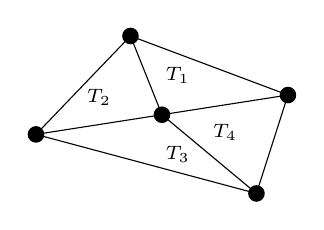
\begin{tikzpicture}
    \def\nv{4}
    \def\ix{1.6}\def\iy{1}
    \def\vertices{
      \coordinate (q0) at (0,0) [label=120:\scriptsize$q_0$];
      \coordinate (q1) at (-\ix*0.25,\iy);
%      \coordinate  (q2) at (-\ix*0.5,\iy);
      \coordinate  (q2) at  (-\ix,-0.25*\iy);
      \coordinate  (q3) at  (0.75*\ix,-\iy);
      \coordinate  (q4) at (\ix*1,0.25*\iy);
    }
    \def\showPoints{
      \foreach \i in {0,...,\nv}
        \fill [black] (q\i) circle (3pt);
    }
    \def\showLines{
      % Draw borders
      \draw (q1) -- (q2) -- (q3) -- (q4) -- cycle;
      % Draw interior edges
      \foreach \i in {1,...,\nv} {
        \draw (q\i) -- (q0);
      }
    }
    \def\showTriangles{
      \node at ($ (q0)!.5!(q1) $) [label=0:\scriptsize${T_1}$] {};
      \node at ($ (q0)!.5!(q2) $) [label=90:\scriptsize${T_2}$] {};
      \node at ($ (q0)!.5!(q3) $) [label=180:\scriptsize${T_3}$] {};
      \node at ($ (q0)!.5!(q4) $) [label=-90:\scriptsize${T_4}$] {};
    }
    \vertices
    \showPoints
    \showLines
    \showTriangles
  \end{tikzpicture}
}

\begin{frame}{Macroelements}
  \small
  \begin{columns}
    \column{0.76\linewidth}
    %---------------------
    \begin{itemize}\itemsep0.1em
      % \item Let $\Uh\sim\Pb$, $\Vh\sim\P1$, $\Ph\sim\P1$ continuous
      %   finite element spaces.
    \item Let $\Th$ a triangulation of $\domain\subset\Rset^2$
    \item Let $\Mh$ a \textbf{macroelement} partition of $\Th$
      \begin{flushright}\scriptsize
        (i.e. a connected sets which is union of at least two
        elements of $\Th$)
      \end{flushright}
    \item We consider macroelements with \alert{one
        only interior vertex}, $q_0$
    \item \textbf{Stenberg Theorem}: Under ``local to global''
      hypothesis, \alert{\textbf{next condition is sufficient for
          inf-sup}}:
    \end{itemize}
    \column{0.3\linewidth}
    %---------------------
    \vtop{\null\hbox{\macroelemA{-0.3}{-0.5}}}
  \end{columns}
 \bigskip
  \begin{equation*}
    \begin{aligned}
      \text{The set $N_M=\left\{ p\in \PM \st \int_M
          \div(u,v)\;p=0, \ \forall (u,v)\in
          \UM\times\VM \right\}$}
      \\[0.66em]
      \text{only consists of the functions which are \textbf{constant} on
        $M$}.
    \end{aligned}
  \end{equation*}
  It is called \textbf{Macro-condition}
%   \medskip
%   \begin{definition}%[\textbf{\amarillo Regular macroelement} condition]
%     In this case, we say \myframed{$M$ is \alert{\textbf{regular}}}
%     for \FEthreeSpaces{\Uh}{\Vh}{\Ph} \quad (or
%     \FEthreeSpaces{\Uh}{\Vh}{\Ph} is \alert{\textbf{regular}})
% %    \vspace{-1em}
%   \end{definition}
\end{frame}


% \begin{frame}{A sufficient condition for discrete Stokes inf-sup}
% %  Let's define:
%   We will use the well known result:
%   \vfill
%   \begin{theorem}[Stenberg'90]
%     Suppose that there is a fixed set of equivalence classes $E_i$ ,
%     $i = 1, 2, ..., l$, of macroelements and a positive integer $L$
%     such that:
%     \begin{description}
%     \item[$(M_1)$] \myframed{Each $M\in E_i$, $i = 1, 2, ..., l$,
%         \textbf{is regular}}
%     \item[$(M_2)$] Each $M \in M_h$ belongs to one of the classes $E_i$ , $i = 1, 2, ..., l$.
%     \item[$(M_3)$] Each interior edge of $\Th$ is interior to at least one and not more than $L$
%     macroelements of $M_h$
%     \end{description}
%     Then Stokes \alert{\textbf{inf-sup condition}} holds.
%   \end{theorem}
% \end{frame}


% \begin{frame}{Macroelements with one only interior vertex}
%   \begin{itemize}\itemsep0.5em
%     \item<1-> We will assume the following \alert{slightly restrictive} hypothesis on \Th:
%       {\it
%       \begin{itemize}
%       \item Each $T\in\Th$ has at least one vertex interior to
%         $\domain$
%       \item $\exists N\in\Nset$ (independ. $h$) s.t. each vertex of
%         $\Th$ is at most in $N$ elements
%       \end{itemize}
%     }
%   \item<2-> Then we will denote by \framedmath<2>{\MhOneVertex} to the macroelement
%     partition defined as follows:
%     \par\vspace{-2em}
%     \begin{tabular*}{0.5\linewidth}{@{\quad}p{0.5\linewidth}p{0.4\linewidth}}
%       \it~\par\vspace{1.5em}  Each $\Macro\in \MhOneVertex$ is union of elements
%       sharing \textbf{one vertex},
%       \framedmath<2>{q_0}
%       \tikz[na] \coordinate(intVertex);
%       &
%       \vtop{\null\hbox{\macroelemA{-0.3}{-0.5}}}
%     \end{tabular*}
%     \vspace{-2em}
%     % \begin{quote}
%     %   Each $\Macro\in \MhOneVertex$ is the union of all the elements
%     %   of $\Th$ sharing one vertex which is interior to $\domain$
%     % \end{quote}
%   \end{itemize}
%   \uncover<3>{
%   \begin{lemma}
%     \label{lemma:macroelements.with.one.interior.vertex}
%     The macroelement partition \MhOneVertex verifies $(M_2)$ and $(M_3)$.
%   \end{lemma}
% %  \smallskip
%   \begin{corollary}
%     If \Th is composed by \textbf{\alert{regular
%       macroelements}} of $\MhOneVertex$
%     % (i.e, $M_1$ \macroCondition holds $\forall
%     % M\in\MhOneVertex$),
%     then
%     \par\hfill\textbf{\alert{inf-sup condition}} holds
%   \end{corollary}
%   }
%   \begin{tikzpicture}[overlay]
%     \path<2>[myarrow] (intVertex) edge [out=0, in=230] (q0);
%   \end{tikzpicture}
% \end{frame}


% \begin{frame}{Structured and unstructured macroelements}
%   We have introduced some definitions:
%   \begin{definition}
%   A macroelement $M$, can be \structure{split by an hyperplane} $\Pi$
%   if there exists two other macroelements $M_1$ and $M_2$ such that:
%   \begin{center}
%     \llaveizq{$M_1\cup M_2=M$  and  \\
%       $M_1\cap M_2 \subset \Pi$}
%     \end{center}
%   \end{definition}

%   \begin{definition}
%     \begin{itemize}
%     \item A macroelement $M$ will be said \structure{\xStructured} if
%       it can be split by an hyperplane $x=C$, for some $C\in\Rset$
%       (i.e. \emph{orthogonal to $OX$ axis})
%     \item In  other case, it will be said \structure{\xUnstructured}
%     \end{itemize}
%   \end{definition}
%   \begin{itemize}
%   \item[$\star$] Analogue definitions for \structure\yUnstructured and
%     \structure\zUnstructured
%   \item[$\star$] For instance...
%   \end{itemize}
% \end{frame}

\newcommand{\bubbleMacro}{ % Bubble macroelement
  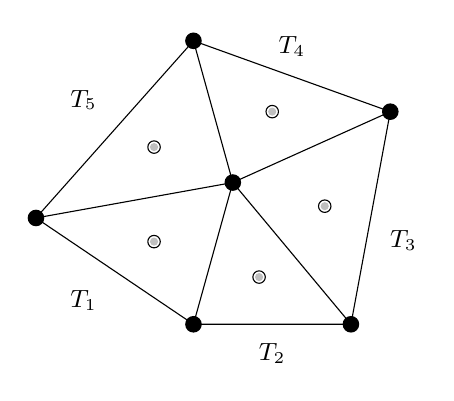
\begin{tikzpicture}
    \def\nv{5}
    \def\ix{2}\def\iy{1.8}
    \def\vertices{
      \coordinate (q0) at (0,0);
      \coordinate (q1) at  (-1.25*\ix,-0.25*\iy);
      \coordinate (q2) at  (-0.25*\ix,-\iy);
      \coordinate (q3) at  (0.75*\ix,-\iy);
      \coordinate (q4) at (\ix*1,0.5*\iy);
      \coordinate (q5) at (-\ix*0.25,\iy);
    }
    \def\showPoints{
      \foreach \i in {0,...,\nv}
      \fill [black] (q\i) circle (3pt);
    }
    \def\showLines{
      % Draw borders
      \draw (q1) -- (q2) -- (q3) -- (q4) -- (q5) -- cycle;
      % Draw interior edges
      \foreach \i in {1,...,\nv} {
        \draw (q\i) -- (q0);
      }
      \foreach \i in {1,...,\nv} {
        \draw [fill, lightgray] (x\i) circle (1.25pt);
        \draw (x\i) circle (2.25pt);
      }
    }
    \def\showTriangles{
      \node at ($ (q1)!.5!(q2) $) [label=230:\small${T_1}$] {};
      \node at ($ (q2)!.5!(q3) $) [label=-90:\small${T_2}$] {};
      \node at ($ (q3)!.5!(q4) $) [label=-15:\small${T_3}$] {};
      \node at ($ (q4)!.5!(q5) $) [label=90:\small${T_4}$] {};
      \node at ($ (q5)!.5!(q1) $) [label=130:\small${T_5}$] {};
    }
    \def\xPoints {
      \coordinate (x1) at ($ (q1)!.5!(q2)!.333!(q0) $);
      \coordinate (x2) at ($ (q2)!.5!(q3)!.333!(q0)  $);
      \coordinate (x3) at ($ (q3)!.5!(q4)!.333!(q0)  $);
      \coordinate (x4) at ($ (q4)!.5!(q5)!.333!(q0)  $);
      \coordinate (x5) at ($ (q1)!.5!(q5)!.333!(q0)  $);
    }
    \vertices
    \xPoints
    \showPoints
    \showLines
    \showTriangles
  \end{tikzpicture}
}


\newcommand{\unstableBubbleMacro}{ % Bubble macroelement where
  % P1b/P1/P1 is unstable
  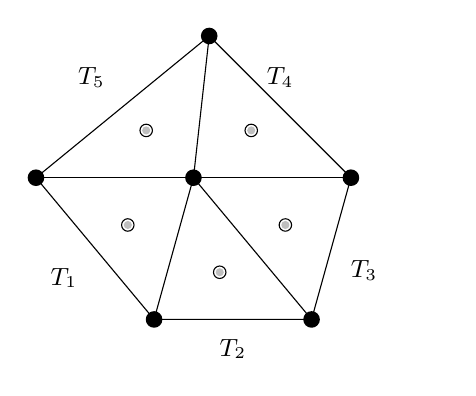
\begin{tikzpicture}
    \def\nv{5}
    \def\ix{2}\def\iy{1.8}
    \def\vertices{
      \coordinate (q0) at (0,0);
      \coordinate (q1) at  (-\ix,0*\iy);
      \coordinate (q2) at  (-0.25*\ix,-\iy);
      \coordinate (q3) at  (0.75*\ix,-\iy);
      \coordinate (q4) at (\ix*1,0*\iy);
      \coordinate (q5) at (\ix*0.1,\iy);
    }
    \def\showPoints{
      \foreach \i in {0,...,\nv}
      \fill [black] (q\i) circle (3pt);
    }
    \def\showLines{
      % Draw borders
      \draw (q1) -- (q2) -- (q3) -- (q4) -- (q5) -- cycle;
      % Draw interior edges
      \foreach \i in {1,...,\nv} {
        \draw (q\i) -- (q0);
      }
      \foreach \i in {1,...,\nv} {
        \draw [fill, lightgray] (x\i) circle (1.25pt);
        \draw (x\i) circle (2.25pt);
      }
    }
    \def\showTriangles{
      \node at ($ (q1)!.5!(q2) $) [label=230:\small${T_1}$] {};
      \node at ($ (q2)!.5!(q3) $) [label=-90:\small${T_2}$] {};
      \node at ($ (q3)!.5!(q4) $) [label=-15:\small${T_3}$] {};
      \node at ($ (q4)!.5!(q5) $) [label=90:\small${T_4}$] {};
      \node at ($ (q5)!.5!(q1) $) [label=130:\small${T_5}$] {};
    }
    \def\xPoints {
      \coordinate (x1) at ($ (q1)!.5!(q2)!.333!(q0) $);
      \coordinate (x2) at ($ (q2)!.5!(q3)!.333!(q0)  $);
      \coordinate (x3) at ($ (q3)!.5!(q4)!.333!(q0)  $);
      \coordinate (x4) at ($ (q4)!.5!(q5)!.333!(q0)  $);
      \coordinate (x5) at ($ (q1)!.5!(q5)!.333!(q0)  $);
    }
    \vertices
    \xPoints
    \showPoints
    \showLines
    \showTriangles
    \node at ($ (q4)!.4!(q5)!-1!(q0) $) {};
    \node at ($ (q4)!.333!(q3)!-0.7!(q0) $) {};
  \end{tikzpicture}
}

\begin{frame}{{\amarillo\xStructured} and {\amarillo\xUnstructured} macroelements}
  \begin{columns}
    \column{0.5\linewidth}
    \unstableBubbleMacro
    \\
    \begin{itemize}
    \item \myframed{\textbf\xUnstructured}
       (it cannot be \structure{split} by any line
      orthogonal to $OX$ axis)
    \item \myframed{\textbf\yStructured}
      \ (can be \structure{split} by a line
      orthogonal to $OY$)
    \end{itemize}
    % --------
    \pause
    \column{0.5\linewidth}
    \bubbleMacro
    \\
    \begin{itemize}
    \item \textbf\xUnstructured\ macroelement
    \item Also \textbf\yUnstructured
    \end{itemize}
    \vspace{1.5em}~
   \end{columns}
\end{frame}

\begin{frame}{Regular macroelements for \FEthreeSpacesP{1,b}11}
  \begin{itemize}\itemsep1em
  \item The following result \colorUnderLine{relates
      \textbf{Macro-condition} with \textbf{structure}}
\item In fact, it states that ~\medskip
  \quad

  \begin{BlockNoTitle}
    \begin{center} \it bubbles can be
      \textbf{\itshape removed from one (only) component of velocity} \\
      \rotatebox{90}{$\Leftrightarrow$}
      \\
      $M$ is \it \ \textbf{\itshape unstructured in corresponding
        direction}
    \end{center}
  \end{BlockNoTitle}

\item More specifically...
  \begin{theorem}
    Let $M$ be a macroelement in $\MhOneVertex$.
    Then
    \begin{center}
      \colorUnderLine{\FEthreeSpacesP{1,b}{1}{1} verifies
        \textbf{Macro-condition} in $M$} $\Leftrightarrow$ $M$ is
      \colorUnderLine{\textbf{\yUnstructured}}
    \end{center}
  \end{theorem}
  \item[$\star$] Analogue result for \FEthreeSpacesP{1}{1,b}{1}
% \item[$\star$] For instance...
\end{itemize}
\end{frame}

% \begin{frame}{{\amarillo Regular} and {\amarillo not regular} macroelements}
%   \small
%   \begin{columns}
%     \column{0.5\linewidth}
%     \unstableBubbleMacro
%     \\
%     \begin{itemize}
%     \item \xUnstructured $\Rightarrow$
%       \par~ \hfill \myframed<1>{\FEthreeSpacesP1{1,b}1 \textbf{Macro-cond.}}
%     \item \yStructured $\Rightarrow$
%       \par~ \hfill \myframed<1>{\FEthreeSpacesP{1,b}11  \textbf{No
%           Macro-cond.}}
%     \end{itemize}
%     \vfill~
%     % --------
%     \pause
%     \column{0.5\linewidth}
%     \bubbleMacro
%     \\
%     \begin{itemize}
%     \item \xUnstructured $\Rightarrow$
%       \par~ \hfill \myframed<2>{\FEthreeSpacesP{1,b}11
%         \textbf{Macro-cond}}
%     \item \yUnstructured $\Rightarrow$
%       % \FEthreeSpacesP1{1,b}1 is  \textbf{regular}
%       \par~ \hfill \myframed{\FEthreeSpacesP1{1,b}1
%         \textbf{Macro-cond}}
%     \end{itemize}
%     \vspace{0.9em}
%    \end{columns}
% \end{frame}

\begin{frame}{Sufficient condition for stability}
  \begin{corollary}
    If a mesh is composed of \textbf{\yUnstructured macroelements}, then
    \alert{inf-sup condition holds for \FEthreeSpacesP{1,b}11} elements
  \end{corollary}
  \begin{center}
     \pgfimage[width=0.9\linewidth,height=7\baselineskip]{\imgdir/mesh-xStr-yUnstr}
  \end{center}
  \begin{itemize}\itemsep0.9em
  \item \textbf{Proof}: Apply Stenberg's Theorem.
  \item Analogue result for \FEthreeSpacesP1{1,b}1
  \end{itemize}
\end{frame}

% \begin{frame}{\myframedAlert{\FEthreeSpacesP{1,b}11 (or Mini-mini-element)}: advantages}
%   \begin{enumerate}[<+->]\itemsep0.5em
%   \item In practice, one can hope \textbf{\alert{inf-sup condition is
%         verified in most meshes}}, specifically those build by
%     \textbf{usual mesh generators}. Our \textbf{numerical tests
%       confirm} this fact
%   \item It can be shown the following \alert{\textbf{optimal error
%         estimates}}:
%     \begin{equation*}
%       \|\ww - \ww_h\|_{H^1} + \| p - p_h\|_{L^2} \le C\, h\quad \hbox{and}\quad
%       \|\ww - \ww_h\|_{L^2} \le C\, h^2
%     \end{equation*}
%     They agree with our \textbf{numerical tests}
%   \item We have found a ``\myframed<3>{\alert{\textbf{\itshape
%           Mini-mini-element}}}'': element
%     \begin{itemize}
%     \item with less d.o.f. than the mini element,
%     \item with optimal order and
%     \item stable in most meshes
%     \end{itemize}

%   % \item Previous theorem is \alert{\textbf{not a necessary condition}}
%   %   and inf-sup condition may be verified even if some $M$ are
%   %   structured
%   \item In fact, \alert{\textbf{counterexamples where inf-sup
%         condition is not verified}} have been found just in meshes having
%     \textbf{both a strong $x$-structure and $y$-structure}
%   \end{enumerate}
% \end{frame}

\begin{frame}{\myframedAlert{Stokes \FEthreeSpacesP{1,b}11}
    lid-driven cavity test, 1}
  \begin{tabular}{@{}c@{}c@{}c@{}}
    \pgfimage[width=0.32\linewidth]{\imgdir/unstruct-mesh}
    &
    \pgfimage[width=0.31\linewidth]{\imgdir/b1-1-v-uns}
    &
    \pgfimage[width=0.31\linewidth]{\imgdir/b1-1-p-uns}
  \end{tabular}
  \textbf{Unstructured mesh}

  \begin{tabular}{@{}c@{}c@{}c@{}}
    \pgfimage[width=0.32\linewidth]{\imgdir/struct-mesh}
    &
    \pgfimage[width=0.31\linewidth]{\imgdir/b1-1-v-str}
    &
    \pgfimage[width=0.31\linewidth]{\imgdir/b1-1-p-str}
  \end{tabular}
  \textbf{Structured mesh} %\FEthreeSpacesP{1,b}{1,b}1
\end{frame}

% \begin{frame}{Mesh structured in just 1 direction}
%   Test in a $x$--structured but $y$--unstructured mesh
%   \begin{center}
    % \pgfimage[width=0.5\linewidth,height=5\baselineskip]{\imgdir/mesh-xStr-yUnstr}
    % \\
  %   \begin{tabular}{@{}c@{}c@{}c@{}}
  %     \pgfimage[width=0.32\linewidth]{\imgdir/bb-1_x-struc_y_unstruct}
  %     &
  %     \pgfimage[width=0.32\linewidth]{\imgdir/b1-1_x-struc_y_unstruct}
  %     &
  %     \pgfimage[width=0.32\linewidth]{\imgdir/1b-1_x-struc_y_unstruct}
  %     \\
  %     \FEthreeSpacesP{1,b}{1,b}1
  %     &
  %     \FEthreeSpacesP{1,b}{1}1
  %     &
  %     \FEthreeSpacesP{1}{1,b}1
  % \end{tabular}
%   \end{center}
% \end{frame}


% \begin{frame}{\myframedAlert{\FEfourSpacesP11{1,b}1} 3D
%     finite elements}
%   ¿Cual de las simulaciones 3D meto?
% \end{frame}

\begin{frame}{\myframedAlert{\FEthreeSpacesP{2}11}
    stability}
  \begin{enumerate}\itemsep0.66em
  \item Methods and results: parallel to \FEthreeSpacesP{1,b}11
    (although more technical)
  \item We have also proved that \FEthreeSpacesP{2}11 is stable in
    most unstructured 2D meshes
  \end{enumerate}
\end{frame}

\begin{frame}{Macro-condition for \FEthreeSpacesP{2}{1}{1}}
  \begin{theorem}
    Let $M$ be a macroelement in $\MhOneVertex$.
    Then \textbf{Macro-condition} is verified for \colorUnderLine{\FEthreeSpacesP{2}{1}{1} is
      in $M$}
    $\Leftrightarrow$ $M$ is
    \colorUnderLine{\textbf{\yUnstructured}} except...

    \begin{quote}
      $\nv$ is even and the following algebraic condition
      holds \vspace{-0.6em} {\scriptsize
        \begin{equation*}
          \label{eq:ch1:instabilityMacroCondition}
          \sum_{i=1}^\nv (-1)^{i} \cot(\sigma_i)\left(\frac1{|T_i|}+ \frac1{|T_{i+1}|} \right) = 0,
        \end{equation*}
      }
      \vspace{-0.6em}
      {\scriptsize
        where $\sigma_i$: angle between positive horizontal
        semiaxis from $q_0$ and  common edge of $T_i$ and $T_{i+1}$
      }
    \end{quote}
  \end{theorem}


\textbf{Proof}: Similar to \FEthreeSpacesP{1,b}{1}{1}, but
more technical \hfill $\square$
\par\mbox{}
\end{frame}

% \begin{frame}
%   \begin{proof}
%     \begin{itemize}
%     \item Es m\'as complicada que \FEthreeSpacesP{1,b}11
%     \item Idea: Usar la de  mi charla para el grupo de Tom\'as
%       (repasarla)
%     \end{itemize}
%   \end{proof}
% \end{frame}

  \newcommand{\macroelemD}{
    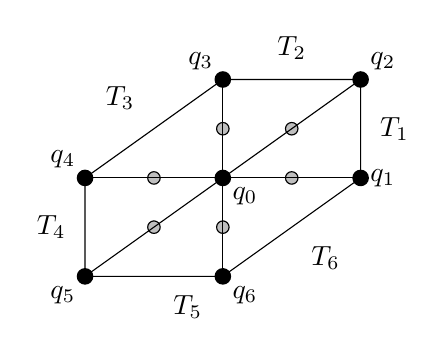
\begin{tikzpicture}
      \def\nv{6}
      \def\ix{1.75}\def\iy{1.25}
      \def\vertices{
        \coordinate [label=-45:$q_0$] (q0) at (0,0);
        \coordinate [label=right: $q_1$] (q1) at (\ix*1,0);
        \coordinate [label=+45: $q_2$] (q2) at (\ix,\iy);
        \coordinate [label=+135: $q_3$] (q3) at  (0,\iy);
        \coordinate [label=+135: $q_4$] (q4) at   (-\ix,0);
        \coordinate [label=225: $q_5$] (q5) at (-\ix,-\iy);
        \coordinate [label=-45: $q_6$] (q6) at (0,-\iy);
      }
      \def\xPoints {
        \coordinate (x1) at ($ (q1)!.5!(q0) $);
        \coordinate (x2) at ($ (q2)!.5!(q0) $);
        \coordinate (x3) at ($ (q3)!.5!(q0) $);
        \coordinate (x4) at ($ (q4)!.5!(q0) $);
        \coordinate (x5) at ($ (q5)!.5!(q0) $);
        \coordinate (x6) at ($ (q6)!.5!(q0) $);
      }
      \def\showPoints{
        \foreach \i in {0,...,\nv}
        \fill [black] (q\i) circle (3pt);
        \foreach \i in {1,...,\nv} {
          \draw [fill, lightgray] (x\i) circle (2.25pt);
          \draw (x\i) circle (2.25pt);
        }
      }
      \def\showLines{
        % Draw borders
        \draw (q1)--(q2) -- (q3) -- (q4) -- (q5) -- (q6) -- cycle;
        % Draw interior edges
        \foreach \i in {1,...,\nv} {
          \draw (q\i) -- (q0);
        }
      }
      \def\showTriangles{
        \node at ($ (q6)!.5!(q1) $) [label=-45:${T_6}$] {};
        \node at ($ (q1)!.5!(q2) $) [label=0:${T_1}$] {};
        \node at ($ (q2)!.5!(q3) $) [label=90:${T_2}$] {};
        \node at ($ (q3)!.5!(q4) $) [label=135:${T_3}$] {};
        \node at ($ (q4)!.5!(q5) $) [label=180:${T_4}$] {};
        \node at ($ (q5)!.5!(q6) $) [label=-45:${T_5}$] {};
      }
      \vertices
      \xPoints
      \showPoints
      \showLines
      \showTriangles
    \end{tikzpicture}
  }
  \newcommand{\macroelemE}{
    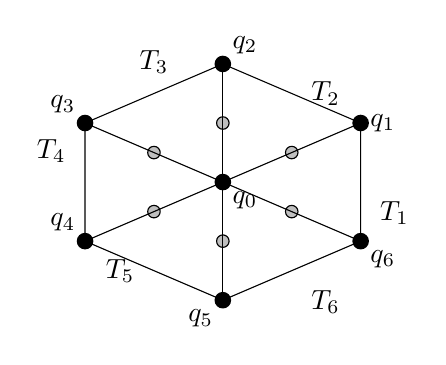
\begin{tikzpicture}
      \def\nv{6}
      \def\ix{1.75}\def\iy{0.75}
      \def\vertices{
        \coordinate [label=-45:$q_0$] (q0) at (0,0);
        \coordinate [label=right: $q_1$] (q1) at (\ix,\iy);
        \coordinate [label=+45: $q_2$] (q2) at (0,2*\iy);
        \coordinate [label=+135: $q_3$] (q3) at  (-\ix,\iy);
        \coordinate [label=+135: $q_4$] (q4) at   (-\ix,-\iy);
        \coordinate [label=225: $q_5$] (q5) at (0,-2*\iy);
        \coordinate [label=-45: $q_6$] (q6) at (\ix,-\iy);
      }
      \def\xPoints {
        \coordinate (x1) at ($ (q1)!.5!(q0) $);
        \coordinate (x2) at ($ (q2)!.5!(q0) $);
        \coordinate (x3) at ($ (q3)!.5!(q0) $);
        \coordinate (x4) at ($ (q4)!.5!(q0) $);
        \coordinate (x5) at ($ (q5)!.5!(q0) $);
        \coordinate (x6) at ($ (q6)!.5!(q0) $);
      }
      \def\showPoints{
        \foreach \i in {0,...,\nv}
        \fill [black] (q\i) circle (3pt);
        \foreach \i in {1,...,\nv} {
          \draw [fill, lightgray] (x\i) circle (2.25pt);
          \draw (x\i) circle (2.25pt);
        }
      }
      \def\showLines{
        % Draw borders
        \draw (q1)--(q2) -- (q3) -- (q4) -- (q5) -- (q6) -- cycle;
        % Draw interior edges
        \foreach \i in {1,...,\nv} {
          \draw (q\i) -- (q0);
        }
      }
      \def\showTriangles{
        \node at ($ (q6)!.5!(q1) $) [label=-45:${T_1}$] {};
        \node at ($ (q1)!.5!(q2) $) [label=0:${T_2}$] {};
        \node at ($ (q2)!.5!(q3) $) [label=90:${T_3}$] {};
        \node at ($ (q3)!.5!(q4) $) [label=135:${T_4}$] {};
        \node at ($ (q4)!.5!(q5) $) [label=180:${T_5}$] {};
        \node at ($ (q5)!.5!(q6) $) [label=-45:${T_6}$] {};
      }
      \vertices
      \xPoints
      \showPoints
      \showLines
      \showTriangles
    \end{tikzpicture}
  }


% \begin{frame}{{\amarillo Not regular} \FEthreeSpacesP211 macroelements}
%   \begin{columns}
%     %- - - - - - - - - - - -
%     \column[t]{0.49\linewidth}
%     %- - - - - - - - - - - -
%     % \subfloat[Two vertices
%     % horizontally aligned with $q_0$.]{
%     \macroelemD
%     \begin{flushleft}
%       \quad\alert{(a)}\quad \myframed{\yStructured}
%     \end{flushleft}
%     % \subfloat[No vertex horizontally aligned, but $n$ is even
%     % and~(\ref{eq:ch1:instabilityMacroCondition}) holds.]{
%     %- - - - - - - - - - - -
%     \column[t]{0.49\linewidth}
%     %- - - - - - - - - - - -
%     \macroelemE
%     \begin{figure}
%       \alert{(b)}\quad \myframed{\yUnstructured}
%       \\[0.66em]
%       (``\textit{weak}'' $y$--structure)
%     \end{figure}
%   \end{columns}
% \end{frame}

\begin{frame}{\myframedAlert{Stokes \FEthreeSpacesP{2}11}
    lid-driven cavity test}
  \begin{center}
    \begin{tabular}{rr}
      \pgfimage[width=0.2\linewidth]{\imgdir/unstruct-mesh}
      &
      \pgfimage[width=0.2\linewidth]{\imgdir/struct-mesh}
      \\[-0.2em]
      \pgfimage[width=0.458\linewidth]{\imgdir/21-1-p-uns}
      &
      \pgfimage[width=0.45\linewidth]{\imgdir/21-1-p-str}
      \\
      \scriptsize Unstructured mesh pressure \quad & \scriptsize Structured mesh pressure\quad
    \end{tabular}
    \par\mbox{}
  \end{center}
\end{frame}

\begin{frame}{Stokes \FEthreeSpacesP{2}11 error orders}
  \small
  \begin{columns}
    % - - - - - - - - - - - - -
    \column{0.50\linewidth}
    % - - - - - - - - - - - - -
    Orders in energy norms:
    \begin{itemize}
    \item<2-> \myframed<2>{$\OO(h^{\mathbf{2}})$ for $\uu$ and $\vv$
        in $\|\cdot\|_{L^2}$}
          \tikz[na] \coordinate(uv-l2-error-L);
    \item<3-> \myframed<3>{$\OO(h^{\mathbf{1}})$ for $\uu$ and $\vv$
        in $\|\cdot\|_{H^1}$}
          \tikz[na] \coordinate(uv-h1-error-L);
        \item<4-> \myframed<4>{$\OO(h^{\mathbf{1}})$ for $\pp$ in $\|\cdot\|_{L^2}$}
          \tikz[na] \coordinate(p-l2-error-L);
      \par\medskip
    % \item Note: Order $\OO(h^3)$ not reached for $\uu\sim\P2$ due to
    %   influence of $\vv\sim\P1$
    \end{itemize}
    % - - - - - - - - - - - - -
    \column{0.49\linewidth}
    % - - - - - - - - - - - - -
   \begin{tikzpicture}
      \node [inner sep=0pt,above right]{
        \pgfimage[width=\linewidth]{\imgdir/21-1-errors-loglog}
      };
      \path (2,2.1) coordinate (u-error-img);
      \path (2,3) coordinate (v-h1z-error-img);
      \path (2,1.8) coordinate (v-l2-error-img);
    \end{tikzpicture}
  \end{columns}
  % - - - - - - - - - - - - - - - - - - - - - - - - - - - - - - - - -
  \vspace{-1em}
  \begin{overprint}
    \begin{center}
      \scriptsize
      \begin{tabular}{l@{\qquad}r@{\qquad}rrrrrr}
        \toprule
        $h_{\max}$ & & $2^{-3}$ & $2^{-4}$ & $2^{-5}$ & $2^{-6}$ & $2^{-7}$
        & $2^{-8}$
        \\ \otoprule
        \multirow{2}*{$\uu$}
        & $\|u-u_h\|_{L^2}$ &
        \rowalert{2} {2.185  }{ 2.291  }{ 2.008} {
          \tikz[na]  \node(u-l2-error-R) {2.029  };
        }{2.031  }{ 2.066}
        \\ \cmidrule{2-8}
        & $\|u-u_h\|_{H^1_0}$ &
        \rowalert{3} {1.758  }{ 1.774  }{ 0.986} {
          \tikz[na]  \node(u-h1-error-R) {1.212};
        }{1.067  }{ 1.237}
        \\ \midrule
        \multirow{2}*{$\vv$}
        & $\|v-v_h\|_{L^2}$ &
        \rowalert{2} {2.056  }{ 2.116  }{ 2.028} { \tikz[na]
          \node(v-l2-error-R) {1.980};  }{ 2.068  }{ 2.040}
        \\ \cmidrule{2-8}
        & $\|\dz v-\dz v_h\|_{L_2}$ &
        \rowalert{3} {0.977  }{ 1.044  }{ 1.017}{ \tikz[na]
          \node(v-h1z-error-R){0.990}; }{1.022  }{ 1.019}
        \\ \midrule
        $\pp$
        & $\|p-p_h\|_{L^2}$ &
        \rowalert{4} {1.070  }{ 2.101  }{ 0.798}{ \tikz[na]
          \node(p-l2-error-R){1.419};}{0.599  }{ 0.820}
        \\ \bottomrule
      \end{tabular}
    \end{center}
  \end{overprint}
  \begin{tikzpicture}[overlay]
    \path<2>[myarrow]
    (u-l2-error-R) edge [in=0,out=155] (uv-l2-error-L);
    % \path<2>[myarrow2]
    % (u-error-L) edge [out=0, in=170] (u-error-img);
    %
    \path<2>[myarrow]
    (v-l2-error-R) edge [in=0,out=155] (uv-l2-error-L);
    % \path<3>[myarrow2]
    % (v-h1z-error-L) edge [out=0, in=170] (v-h1z-error-img);
    % ------------------------------------------------------
    \path<3>[myarrow]
    (u-h1-error-R) edge [out=155, in=0] (uv-h1-error-L);
    %
    % \path<2>[myarrow2]
    % (u-error-L) edge [out=0, in=170] (u-error-img);
    \path<3>[myarrow]
    (v-h1z-error-R) edge [out=155, in=0] (uv-h1-error-L);
    % \path<3>[myarrow2]
    % (v-h1z-error-L) edge [out=0, in=170] (v-h1z-error-img);
    % ------------------------------------------------------
    \path<4>[myarrow]
    (p-l2-error-R) edge [out=155, in=0] (p-l2-error-L);
    % \path<4>[myarrow2]
    % (p-l2-error-L) edge [out=0, in=155] (v-l2-error-img);
  \end{tikzpicture}
\end{frame}


\begin{frame}{3D finite elements}

  Similar results are shown in \textbf{3D} when one delete \textbf{bubbles}...
  \begin{itemize}\itemsep0.7em
  \item \FEfourSpacesP{1,b}{1,b}{1}{1}
  \item \FEfourSpacesP{1,b}{1}{1}{1}
  \end{itemize}

  \medskip
  And also when one delete degrees of freedom in \textbf{3D Taylor-Hood} elements
  \begin{itemize}\itemsep0.7em
  \item  \FEfourSpacesP{2}{2}{1}{1}
  \item \FEfourSpacesP{2}{1}{1}{1}
  \end{itemize}
  \bigskip
  \textbf{Proof}: Similar 2D but quite technical in some cases \hfill $\square$
\end{frame}

\begin{frame}{3D tests (lid-driven cavity tests)}

  \textbf{Structured mesh}
  \begin{tabular}{ccc}
    \pgfimage[width=0.3\linewidth]{\imgdir/222-1-str}
    &
    \pgfimage[width=0.3\linewidth]{\imgdir/221-1-str}
    &
    \pgfimage[width=0.3\linewidth]{\imgdir/211-1-str}
  \end{tabular}
  \textbf{Unstructured mesh}
  \begin{tabular}{ccc}
    \pgfimage[width=0.3\linewidth]{\imgdir/222-1-uns}
    &
    \pgfimage[width=0.3\linewidth]{\imgdir/221-1-uns}
    &
    \pgfimage[width=0.3\linewidth]{\imgdir/211-1-uns}
    \\[-0.3em]
    \small\FEfourSpacesP2221 & \small\FEfourSpacesP2211 &
    \small\FEfourSpacesP2111
  \end{tabular}
\end{frame}



%%% Local Variables:
%%% coding: utf-8
%%% TeX-master: "numerical-oceanography"
%%% mode: latex
%%% ispell-local-dictionary: "english"
%%% End:


% %%,---------------------------------------------------------------------
% %%| Stokes with Unequal FE for Velocity
% %%`---------------------------------------------------------------------
% \section{Stokes with Unequal FE for Velocity}

%%,---------------------------------------------------------------------
%%| Hydrostatic Stable FE combinations}
%%`---------------------------------------------------------------------
\section{Hydrostatic Stable FE Combinations}
\label{sec:hydr-stable-fe}
% \include{sec-hydrstokes-stability}
% \include{sec-stokes}
% \include{sec-hydrstokes-tests}

%%,---------------------------------------------------------------------
%%|
%%`---------------------------------------------------------------------
\section{Stabilized Reformulations of Hydrostatic Stokes}
\label{sec:stab-reform-hydr}
% \include{sec-v-stabilized}

%%,---------------------------------------------------------------------
%%| Time schemes and variable denisity
%%`---------------------------------------------------------------------
\section{Time integration of the whole set of equations}
\label{sec:time-integr-whole}
% \include{sec-vardens-time}


%%,---------------------------------------------------------------------
%%| Conclusions and future work
%%`---------------------------------------------------------------------
\begin{frame}{Conclusions}
  \begin{itemize}\itemsep0.66em
  \item<1-> We have developed \alert{new schemes} for approximation of
    Primitive Equations of the Ocean (or even Anisotropic Navier-Stokes)
    \begin{itemize}
    \item Avoiding velocity instabilities of (quasi-)hydrostatic
      formulations
    \end{itemize}
  \item<2-> \alert{Standard FE tools and techniques} like mesh adaptation
    can be used, in \alert{more general meshes} than previous schemes
  \item<3-> Two different approached have been followed:
    \begin{itemize}
    \item New \alert{stable combinations of FE} (unequal
      approximation of velocity components)
    \item Reformulation of space schemes, \alert{stabilizing vertical
      velocity}. Hence standard Stokes--stable FE can be applied
    \end{itemize}
  \item<4-> Successfully applied to \alert{time-dependent problems},
    including \alert{variable density} and \alert{new time splitting}
    schemes
  \end{itemize}
  \uncover<5>{
  \begin{center}\it
    {In short, we have successfully introduced \textbf{a new approach}\\
    for modelling \textbf{realistic hydrostatic and quasi-hydrostatic fluids},\\
    justifying it both \textbf{analytically and numerically}.
  }
\end{center}
}

\end{frame}
\begin{frame}{~}
  \bigskip
  \Large Thank you for your attention.
  \vfill~
  \begin{flushright}
    \pgfsetfillopacity{0.4}
    \pgfimage[width=0.9\textwidth]{img/gibraltar-velocity-2d-difumin}
  \end{flushright}
\end{frame}

%%,-------------
%%| Bibliography
%%`-------------

\setbeamertemplate{footline}[default]

\begin{frame}[allowframebreaks]{Bibliography}
\bibliographystyle{alpha}
%\bibliographystyle{abbrvnat}
\bibliography{biblio-short.bib}
\end{frame}

\end{document}


%%% Local Variables:
%%% coding: utf-8
%%% TeX-master: t
%%% mode: latex
%%% ispell-local-dictionary: "english"
%%% End:
